\documentclass{article}
\usepackage[utf8]{inputenc}
\usepackage[english]{babel}
\usepackage{lastpage}
\usepackage{float}
\usepackage{natbib}
\usepackage{graphicx}
\usepackage[margin=1.1in]{geometry}
\usepackage{listings} 
\usepackage{watermark}
\usepackage{blindtext}
\usepackage{amsmath}
\usepackage{amssymb}
\usepackage{footnote}
\usepackage{caption}
\usepackage{textcomp}
\makesavenoteenv{table}
\usepackage[table,xcdraw,svgnames]{xcolor}
\usepackage[bottom]{footmisc}
\usepackage{subcaption}
\usepackage[justification=centering]{caption}
\usepackage{subfiles}
\usepackage{mcode}
\usepackage{enumerate}
\usepackage{wrapfig}
\usepackage{fancyhdr}
\usepackage{hyperref}
\usepackage{bm}
\usepackage{makecell}
\usepackage{changepage}
\renewcommand{\baselinestretch}{1.4}
\newcommand{\ts}{\textsuperscript}
\pagestyle{fancy}

%%% DAVIDs tilføjelser:
\bibliographystyle{ieeetr}
\setlength{\parindent}{0pt}
% Bibliography (references)
\usepackage[backend=biber,
            %backref=true,
            abbreviate=false,
            sortcites=ynt,
            sorting=nyt,
            dateabbrev=false,
            alldates=long]{biblatex}
\addbibresource{references.bib}
%\lhead{Scientific Computing}

\rhead{02686 Scientific Computing for Differential Equations}


\linespread{1.3} % Line spacing

%\setlength\parindent{0pt} % Uncomment to remove all indentation from paragraphs

\graphicspath{{./Fig/}} % Specifies the directory where pictures are stored

\usepackage{geometry}
 \geometry{
 a4paper,
 total={170mm,257mm},
 left=30mm,
 right=30mm,
 top=30mm,
 bottom=20mm
 }
 
\begin{document}

%\renewcommand{\headrulewidth}{0.4pt} %header


\cfoot{\thepage\ of \pageref{LastPage}}
%-------------------------------------------------------------------------------
%	TITLE PAGE
%-------------------------------------------------------------------------------
\begin{titlepage}

\newcommand{\HRule}{\rule{\linewidth}{0.5mm}} % Defines a new command for the horizontal lines, change thickness here

\center % Center everything on the page


\includegraphics[width=0.15\textwidth]{Logo/DTU-logo.pdf}
%\quad \quad \quad \quad \quad
%\includegraphics[width=0.2\textwidth]{KUlogo.png}
\\[1cm]


\textsc{\large 02686 - Scientific Computing for Differential Equations }\\[0.5cm] % Minor heading such as course title

%\textsc{\large \bfseries Tennis Major Tournament Match Statistics}\\[0.5cm]

\HRule \\[0.8cm]
{ \huge \bfseries Comparison of Numerical Solvers
}\\[0.4cm] % Title of your document
\HRule \\[1cm]

\begin{minipage}{0.4\textwidth}
\begin{center} \footnotesize
\emph{Author:}\\
David Ribberholt Ipsen (s164522)\\
\end{center}
\end{minipage}\\[4cm]

{\large 
\today %dato 
}
\\[0.2cm] % Date, change the \today to a set date if you want to be precise
\thiswatermark{\centering \put(-180,-720){
\includegraphics[scale=0.55]{Logo/DTU-frise-SH-15.pdf}} }
\end{titlepage}

\newpage
\tableofcontents

\newpage

%-------------------------------------------------------------------------------
%	Problem statement
%-------------------------------------------------------------------------------
\section{Test equation for ODEs}
Considering the test equation

$$
\dot{x}(t)=\lambda x(t), \quad x(0)=x_{0} \label{eq:test}
$$
for $\lambda=-1$ and $x_{0}=1$.

\subsection{Analytical solution}
It is is function that differentiated gives itself times a constant. Therefore for obtaining the analyical solution, try a guess with:
$$
x(t) = \exp(\lambda t)
$$
Then
$$
x'(t) = \lambda \exp(\lambda t) = \lambda x(t)t  \quad \qed
$$
I.e. the analytical solution is $x(t) = \exp(\lambda t)$.

\subsection{Local and global truncation error}
In order to calculate the local and global truncation error, the exact analytical solution to the ODE is required to be known. For that reason, the \textit{test equation} is typically used to \textit{test} the performance of numerical methods. The errors are calculated as follows \cite{JrgensenScientificEquations}:

\textbf{Global error}
$$
e_{k}=x_{k}-x\left(t_{k}\right)
$$
where $x_{k}$ is the numerical (descretized) solution and $x\left(t_{k}\right)$ is the exact (continuous) solution. The global error is thus the accumulated error over time. Therefore, it is commonly calculated in the last step.
\\

\textbf{Local error}
$$
l_{k}=x_{k}-x_{k-1}\left(t_{k}\right)
$$
where $x_{k}$ is the numerical solution and $x_{k-1}\left(t_{k}\right)$ is the analytical one-step solution starting from $x\left(t_{k-1}\right)=x_{k-1}$. Therefore, it is commonly calculated in the first step.
\\

\subsection{Computation of local and global truncation erros}

Now, it is of interest to calculate the error of the following three numerical methods
\\

\textbf{Explicit Euler \cite{JrgensenScientificEquationsb}}
\begin{equation}
    x_{k+1}=x_{k}+\Delta t f\left(t_{k}, x_{k}\right)
\end{equation}

Which intuitively takes a step forward with the current $\dot{x}(t_k) = f(t_k,x_k)$.
\\
\textbf{Implicit Euler \cite{JrgensenScientificEquationsb}}
\begin{equation}
    x_{k+1}=x_{k}+\Delta t f\left(t_{k+1}, x_{k+1}\right)
\end{equation}

Which intuitively takes a step backward with the following $\dot{x}(t_{k+1}) =  f(t_{k+1},x_{k+1})$ as estimated by Newton's Method [ibid.].
\\
\textbf{Classical Runge-Kutta \cite{JrgensenRunge-KuttaEquations}}
$$
\begin{aligned}
T_{1} &=t_{n} & X_{1} &=x_{n} \\
T_{2} &=t_{n}+\frac{1}{2} h & X_{2} &=x_{n}+h \frac{1}{2} f\left(T_{1}, X_{1}\right) \\
T_{3} &=t_{n}+\frac{1}{2} h & X_{3} &=x_{n}+h \frac{1}{2} f\left(T_{2}, X_{2}\right) \\
T_{4} &=t_{n}+h & X_{4} &=x_{n}+h f\left(T_{3}, X_{3}\right) \\
 t_{n+1}=t_{n}+h & & \\
 x_{n+1}=x_{n}+h &\left(\frac{1}{6} f\left(T_{1}, X_{1}\right)+\frac{1}{3} f\left(T_{2}, X_{2}\right)+\frac{1}{3} f\left(T_{3}, X_{3}\right)+\frac{1}{6} f\left(T_{4}, X_{4}\right)\right)
\end{aligned}
$$

Which intuitively takes a full step forward by taking 4 well-timed middle steps and calculating a weighted-average of those.
\\

The results are illustrated in the following two sections.






\subsection{Local error}
From Figure \ref{fig:1_4} it is clear that the Classical Runge-Kutta method is much more precise (on the test equation). In terms of order, a method is said to be of order p if $l_{k}=\mathcal{O}\left(h_{k}^{p+1}\right)$ \cite{JrgensenScientificEquationsc}. The \textit{order} is referring to the number of terms in the Taylor-expansion used to approximate $x_{k+1}$ from $x_k$.

By calculating the slopes of the linear line in the log-log plot we obtain:
$$
a_{Exp} = 2.00, \quad a_{Imp} = 1.98, \quad a_{RK} = 5.00
$$

Corresponding to orders
$$
p_{Exp} = 1, \quad p_{Imp} = 1, \quad p_{RK} = 4
$$


\begin{figure}[H]
    \centering
    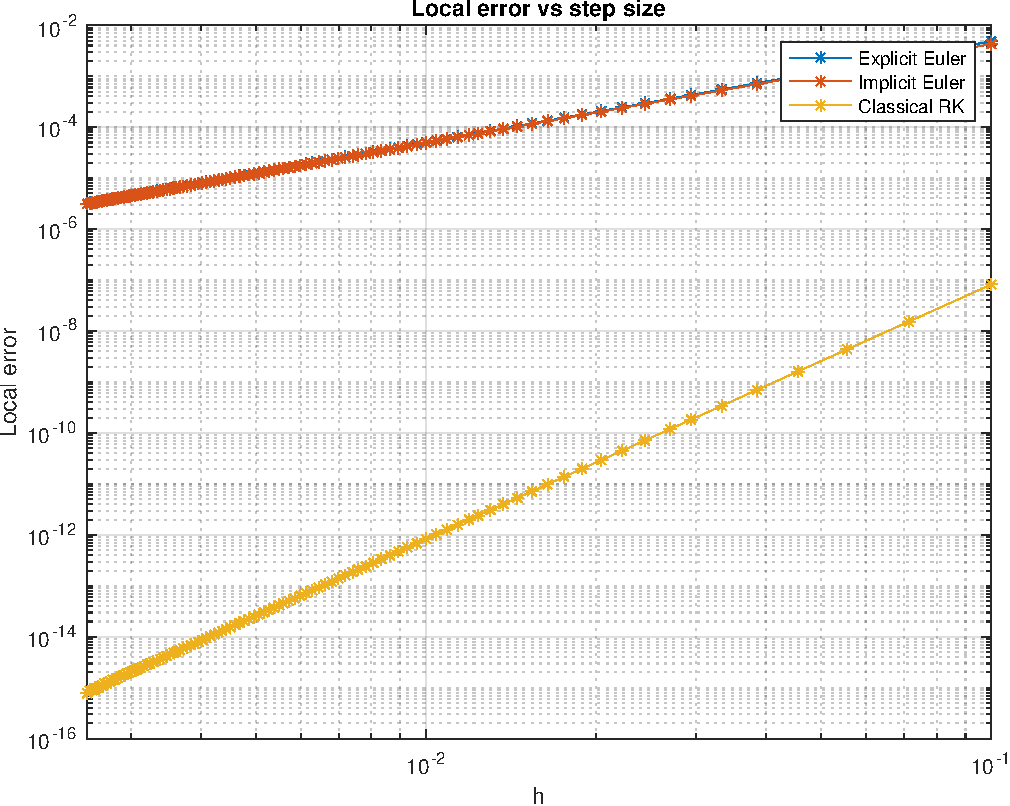
\includegraphics[width=0.7\textwidth]{plots/1_4.pdf}
    \caption{Local error vs step size for three numerical ODE solvers.}
    \label{fig:1_4}
\end{figure}



\subsection{Global error}
Similarly, the global error at $t=1.0$ for the three methods is seen in Figure \ref{fig:1_5}.

\begin{figure}[H]
    \centering
    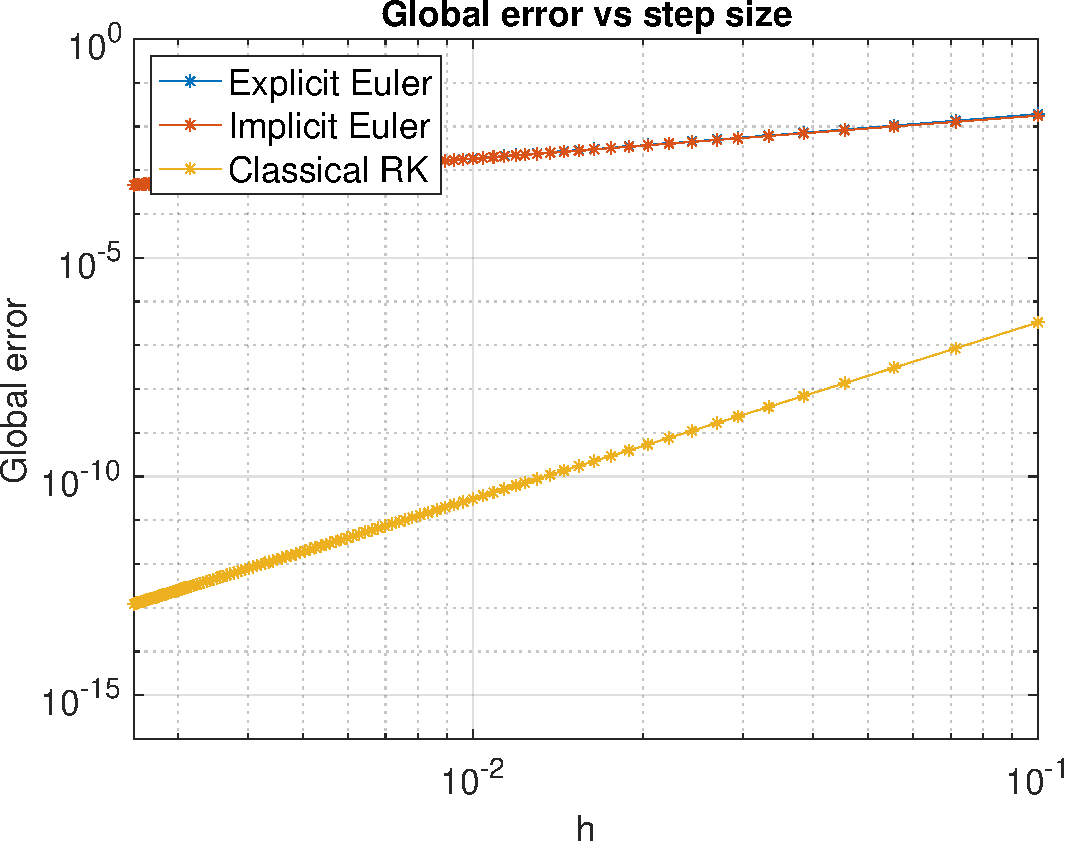
\includegraphics[width=0.7\textwidth]{plots/1_5.pdf}
    \caption{Global error vs step size for three numerical ODE solvers.}
    \label{fig:1_5}
\end{figure}

Again a close to identical performance is seen for the two 1st order methods with the Classical Runge-Kutta being much more accurate. The slopes are

$$
a_{Exp} = 1.00, \quad a_{Imp} = 0.99, \quad a_{RK} = 4.01
$$

Clearly, the global error is proportional to $h_{k}^{p}$, whereas the local error was proportional to $h_{k}^{p+1}$.

\subsection{Stability}
Stability of a methods relates to the \textit{transfer function} $R(z)$ in

\begin{equation}
    x_{k+1}=R(z) x_{k}
\end{equation}

The \textit{stability region} is then defined as \cite{JrgensenScientificEquationsc}
$$ \mathcal{D}=\{z \in \mathbb{C}:|R(z)|<1\} $$

Where $z = \lambda h$, such that if $R(z) > 1$ the method is unstable because the approximation $x_{k+1} \to \infty$ for $k \to \infty$ which is particularly erroneous for cases where $\lambda < 0$ of which the test equation is strictly decreasing. This later case is more formally called \textit{A-stable} [ibid.].

So for a method to be\textit{ A-stable}, it is has to fulfil \cite{JrgensenRunge-KuttaControl}:
\begin{equation}
    \forall z \operatorname{Re}(z)<0  :   |R(z)|<1
\end{equation}

In other words, the method is A-stable if there for all values of z where the real part is below 0 (\iff $\lambda < 0$ since the step size $h > 0$) the \textit{transfer function} is (numerically) below 1.
\\

For a method to be \textit{L-stable} it additionally has to fulfil:
\begin{equation}
\lim _{z \rightarrow-\infty}|R(z)|=0
\end{equation}

I.e. the \textit{transfer function} goes towards 0 when the step size times $\lambda$ goes towards -$\infty$.

\subsubsection*{Deriving stability regions}

Explicit Euler:

Implicit Euler

Classic Runge-Kutta:

[INSERT NOTES MANGLER]


\subsubsection*{Illustrating the stability regions}
The stability regions of the three methods is illustrated in Figure \ref{fig:figure3}. Referring to the definitions above it is seen that none of the methods are A-stable - and thus neither L-stable [TRUE?].

\begin{figure}[htp]
\centering
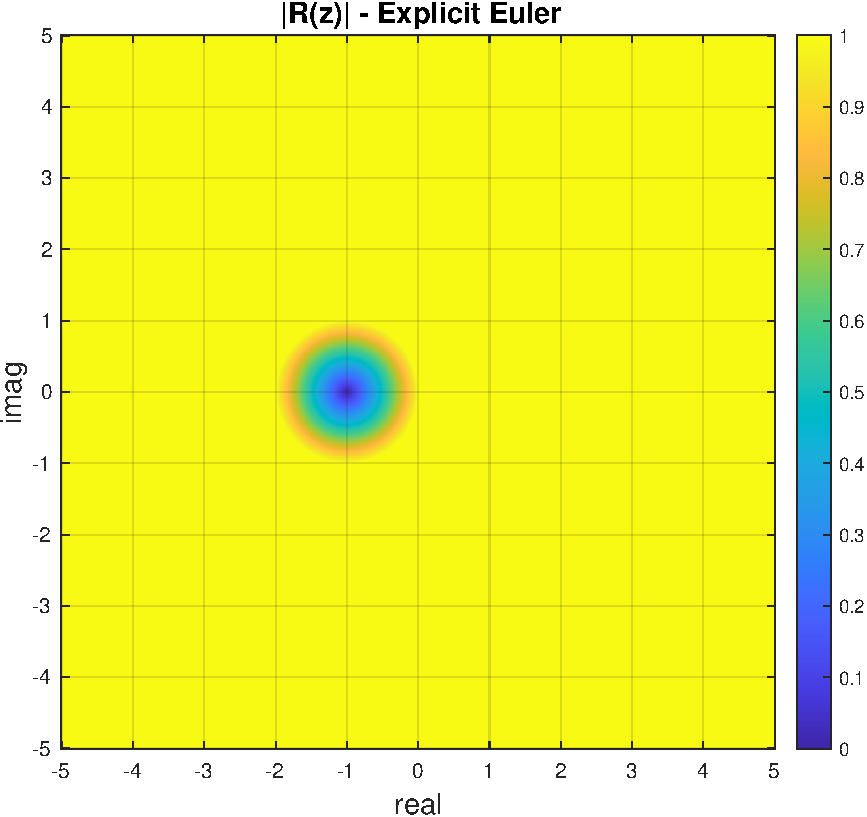
\includegraphics[width=.3\textwidth]{plots/1_6b.pdf}\hfill
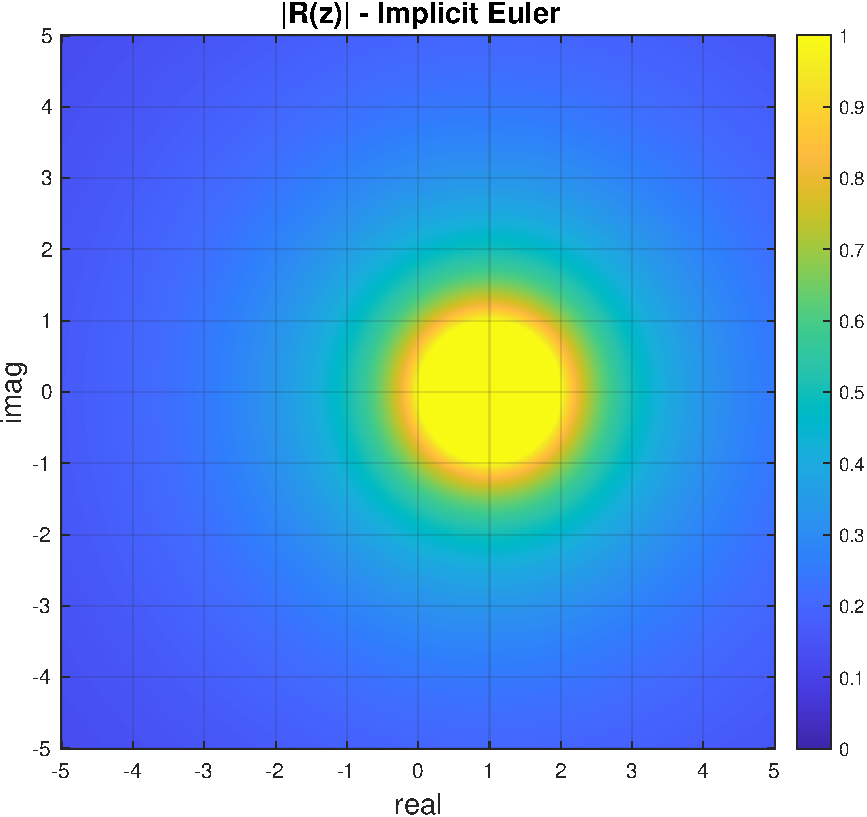
\includegraphics[width=.3\textwidth]{plots/1_6c.pdf}\hfill
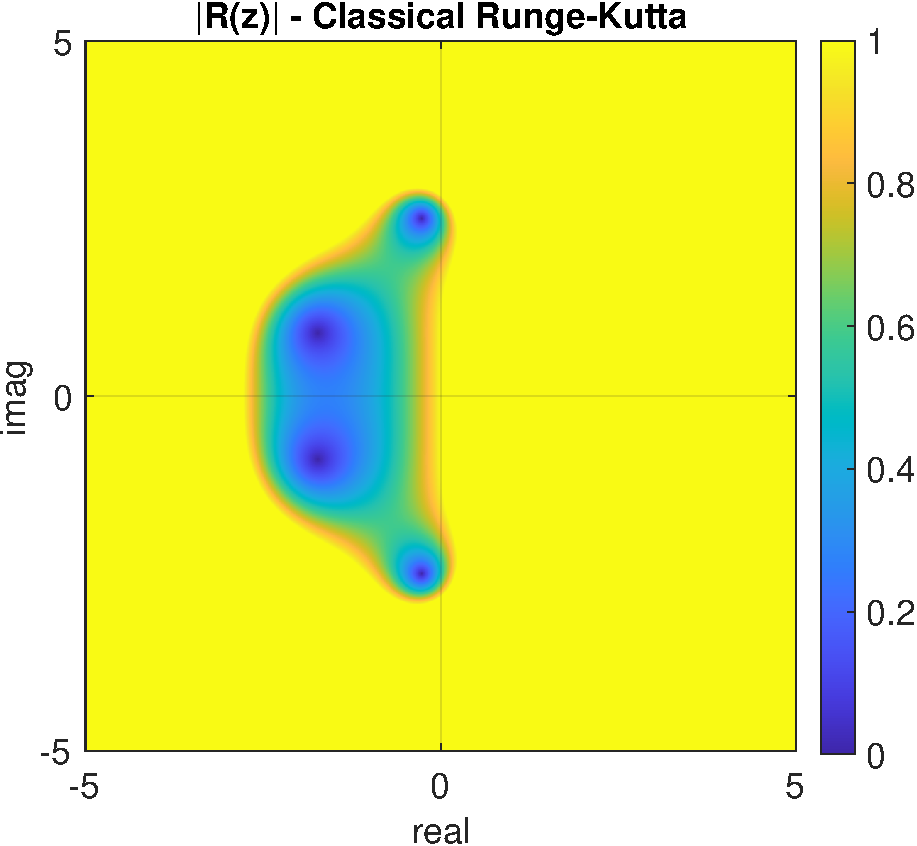
\includegraphics[width=.3\textwidth]{plots/1_6a.pdf}
\caption{Stability regions of the three numerical methods.}
\label{fig:figure3}
\end{figure}
\clearpage
\section{Explicit ODE solver}
\clearpage
\section{Impicit ODE solver}
Considering again the \textit{Initial Value Problem}.
$$
\frac{d}{d t} x(t)= \dot{x}(t)=f(t, x(t), p), \quad x\left(t_{0}\right)=x_{0},
$$
where $x \in \mathbb{R}^{n_{x}}$ and $p \in \mathbb{R}^{n_{p}}$. In the following equations the parameters p are implicit in $f(t, x(t)) = f(t, x(t), p)$.

\subsection{Implicit Euler}
Whereas the Explicit Euler intuitively takes a discrete step forward with $\dot{x}_k$, the Implicit Euler intuitively takes a step \textit{backward} with $\dot{x}_{k+1}$ in each iteration \textit{k} \cite{JrgensenScientificEquationsb}:

\begin{equation}
    x_{k+1}=x_{k}+\Delta t_k f\left(t_{k+1}, x_{k+1}\right)
\end{equation}

Where $\Delta t_k$ is the step size in iteration \textit{k}. It discretises the continuous ODE in the same fashion as the Explicit Euler. The method is analogous to taking the tangent in $x(t_{k+1}) = x_{k+1}$ and taking a $\Delta t_k$ step along the tangent:

\begin{equation}
\frac{x\left(t_{k+1}\right)-x\left(t_{k}\right)}{\Delta t_{k}} \approx \frac{d}{d t} x\left(t_{k+1}\right)=f\left(t_{k+1}, x\left(t_{k+1}\right)\right)
\end{equation}

One natural hurdle arises: We don't know the $\dot{x}_{k+1} = f\left(t_{k+1}, x\left(t_{k+1}\right)\right) = f\left(t_{k+1}, x_{k+1}\right)$ because $x_{k+1}$ is unknown (it is the one we wish to calculate in iteration \textit{k}). Solution: Estimate it using \textit{Newton's method}.

\\\

\textbf{Newton's Method} \\
Newton's method finds the root of a residual function $R(x_{k+1})=0$ using a 1st order Taylor expansion at $x_{k+1}$:
\begin{equation}
    R(x_{k+1}) \approx R(x_k) + \frac{\partial R}{\partial x}\left(x_{k
    }\right)\left(x_{k+1} - x_{k}\right)
\end{equation}

Which can be solved as a linear system of equations \cite{JrgensenScientificEquationsb}. So by formulating the Implicit Euler problem as a residual function: 

\begin{equation}
R\left(x_{k+1}\right)=x_{k+1}-\Delta t f\left(t_{k+1}, x_{k+1}\right)-x_{k}=0
\end{equation}

One can implicitly estimate $x_{k+1}$ by minimising the residual function. In practice, one chooses a tolerance $\epsilon$ for criteria of convergence where $\|R(x)\|_{\infty} \leq \epsilon$ or if a maximum number of iterations has been reached. Using the linear systems formulation, the function is then minimised by Newton's Method by iterating over

$$
\begin{aligned}
&M \Delta x_{k+1}=R\left(x_{k+1}^{[l]}\right) \\
&x_{k+1}^{[l+1]}=x_{k+1}^{[l]}-\Delta x
\end{aligned}
$$

in each iteration \textit{l} where $M=\frac{\partial R}{\partial x}\left(x_{k+1}\right)$ [ibid.]. A decent initial guess at $l=0$ is the simple Explicit Euler step:

$$
x_{k+1}^{[0]}=x_{k}+\Delta t_k f\left(t_{k}, x_{k}\right)
$$

\\\

As with the Explicit Euler, a question arises on choosing an appropriate step size $\Delta t_k$. This gives rise to Implicit Euler with fixed step size:

\begin{equation*}
    \Delta t_k = \Delta t = h \quad \forall_k
\end{equation*}

or Implicit Euler with adaptive step size where $\Delta t_k$ changes in each iteration k. The ladder approach is discussed in further detail in Section 3.3.













\subsection{MATLAB implementation fixed step size}
See the following MATLAB implementation of the Implicit Euler with fixed step size (as described in Section 3.1), well-suited for non-stiff problems.

\begin{adjustwidth*}{0cm}{-0.4cm}
\begin{lstlisting}[frame=single, language=Matlab,caption=Implicit Euler (fixed step size), label=ImplicittEulerFixie]
function [T,X] = ImplicitEulerFixedStepSize(funJac,ta,tb,N,xa,varargin)
    % Compute step size and allocate memory
    dt = (tb-ta)/N;
    nx = size(xa,1);
    X = zeros(nx,N+1);
    T = zeros(1,N+1);

    tol = 1.0e-8;
    maxit = 100;
    % Eulers Implicit Method
    T(:,1) = ta;
    X(:,1) = xa;
    for k=1:N
        [f, J] = feval(funJac,T(k),X(:,k),varargin{:}); T(:,k+1) = T(:,k) + dt;
        xinit = X(:,k) + f*dt;
        X(:,k+1) = NewtonsMethodODE(funJac,...
            T(:,k), X(:,k), dt, xinit, tol, maxit, varargin{:});
    end
    % Form a nice table for the result
    T=T';
    X=X';
end
\end{lstlisting}
\end{adjustwidth*}

Which utilises Newton's Method:

\begin{adjustwidth*}{0cm}{-0.4cm}
\begin{lstlisting}[frame=single, language=Matlab,caption=Newton's Method, label=Newton]
function x = NewtonsMethodODE(FunJac, tk, xk, dt, xinit, tol, maxit, varargin)
    k=0;
    t=tk+dt;
    x = xinit;
    [f,J] = feval(FunJac,t,x,varargin{:});
    R=x-f*dt-xk;
    I = eye(length(xk));
    while( (k < maxit) & (norm(R,'inf') > tol) )
        k=k+1;
        dRdx=I-J*dt;
        dx = dRdx\R;
        x=x-dx;
        [f,J] = feval(FunJac,t,x,varargin{:});
        R=x-dt*f-xk;
    end
end
\end{lstlisting}
\end{adjustwidth*}















\subsection{MATLAB implementation adaptive step size}
See the following MATLAB implementation of the Implicit Euler with adaptive step size, well-suited for stiff and non-stiff problems. The embedded error estimation is based on \textit{stop doubling}, i.e. estimating the error of a full step from the more accurate two half-steps. This procedure has been explained in full detail in Section \ref{sec:ExplicitEulerAdaptive}.

\begin{adjustwidth*}{0cm}{-0.4cm}
\begin{lstlisting}[frame=single, language=Matlab,caption=Implicit Euler (adaptive step size), label=ExplicitEulerFixie]
function [T,X,iter] = ImplicitEulerAdaptiveStep(...
    funJac,tspan,x0,h0,abstol,reltol,varargin)
epstol = 0.8;
facmin = 0.1;
facmax = 5.0;

t0 = tspan(1);
tf = tspan(2);

iter = 0;
% Initial condtions
t = t0;
h = h0; % = dt (step size - bliver modificeret)
x = x0;

% Output
T = t;
X = x';

% Newton syuff
tol = 1e-05;
maxit = 1000;

%% Main algorithm
while t < tf
    iter = iter +1;
    if (t + h >tf)
        h = tf-t;
    end
    f = feval(funJac,t,x,varargin{:});
    AcceptStep = false;
    while ~AcceptStep
        %Take step of size h
        xinit = x + h*f; % Gæt på x+1
        x1 = NewtonsMethodODE(funJac, t, x, h, xinit, tol, maxit, varargin{:});

        %Take step of size h/2
        hm = 0.5*h;
        xinitm = x + hm*f;
        tm = t + hm;

        xm = NewtonsMethodODE(funJac, tm, x, hm, xinitm, tol, maxit, varargin{:});
        
        xinitm2 = x + 2*hm*f ; % = xinit (og derfor redundant)
        x1hat = NewtonsMethodODE(funJac, tm, xm, hm, xinitm2, tol, maxit, varargin{:});

        % Error estimation
        e = x1hat-x1; % Estimate of global error
        r = max(abs(e) ./ max(abstol,abs(x1hat).*reltol));

        AcceptStep = (r <= 1.0);
        if AcceptStep
            t = t+h;
            x = x1hat;

            T = [T;t];
            X = [X;x'];
        end
        % Asymptotic step size controller
        h = max(facmin, min(sqrt(epstol/r), facmax))*h;
    end
end
\end{lstlisting}
\end{adjustwidth*}










\subsection{Van der Pol}


The phase potraits as obtained by solving the Van der Pol problem using the Adaptive Explicit Euler and Fixed (step size) Explicit Euler is seen in Figure \ref{fig:2_4a} and \ref{fig:2_4b}. The problem is solved for t = [0, 32] with $\mu = 3$ and $\mu =20$. Tolerances chosen are $reltol = abstol = \{10^{-2}, 10^{-4}, 10^{-6}\}$. Now a natural question arises, which fixed step sizes $h$ should be chosen for comparison with the adaptive method? The fixed step size $h$ was chosen to result in same number of steps as for the adaptive solution for comparison purposes.

\\
Clearly, for the stiff problem ($\mu = 20$) the fixed step size $h \approx 0.1$ is infeasible. The method is unstable and explodes towards $\infty$ (Figure \ref{fig:2_4a}). For the non-stiff problem ($\mu = 3$), the $h \approx 0.1$ is biased compared to the adaptive methods.
\\

When looking at tolerances of $\{10^{-4}, 10^{-6}\}$ seen in Figure \ref{fig:2_4b} the fixed step size is a lot more accurate, albeit a small bias in the non-stiff problem. For the stiff-problem $h=\frac{1612}{32}$ is very biased and only slightly biased for $h=\frac{14411}{32}$. There is no distinguishable difference between the Adaptive Euler and ode45/ode15s for tolerances $\geq 10^{-4}$.
\\

Note however that the Adaptive Explicit Euler uses a lot more function evaluations than the Fixed Explicit Euler. The choice is a trade-off between speed and accuracy.

\begin{figure}
    \centering
    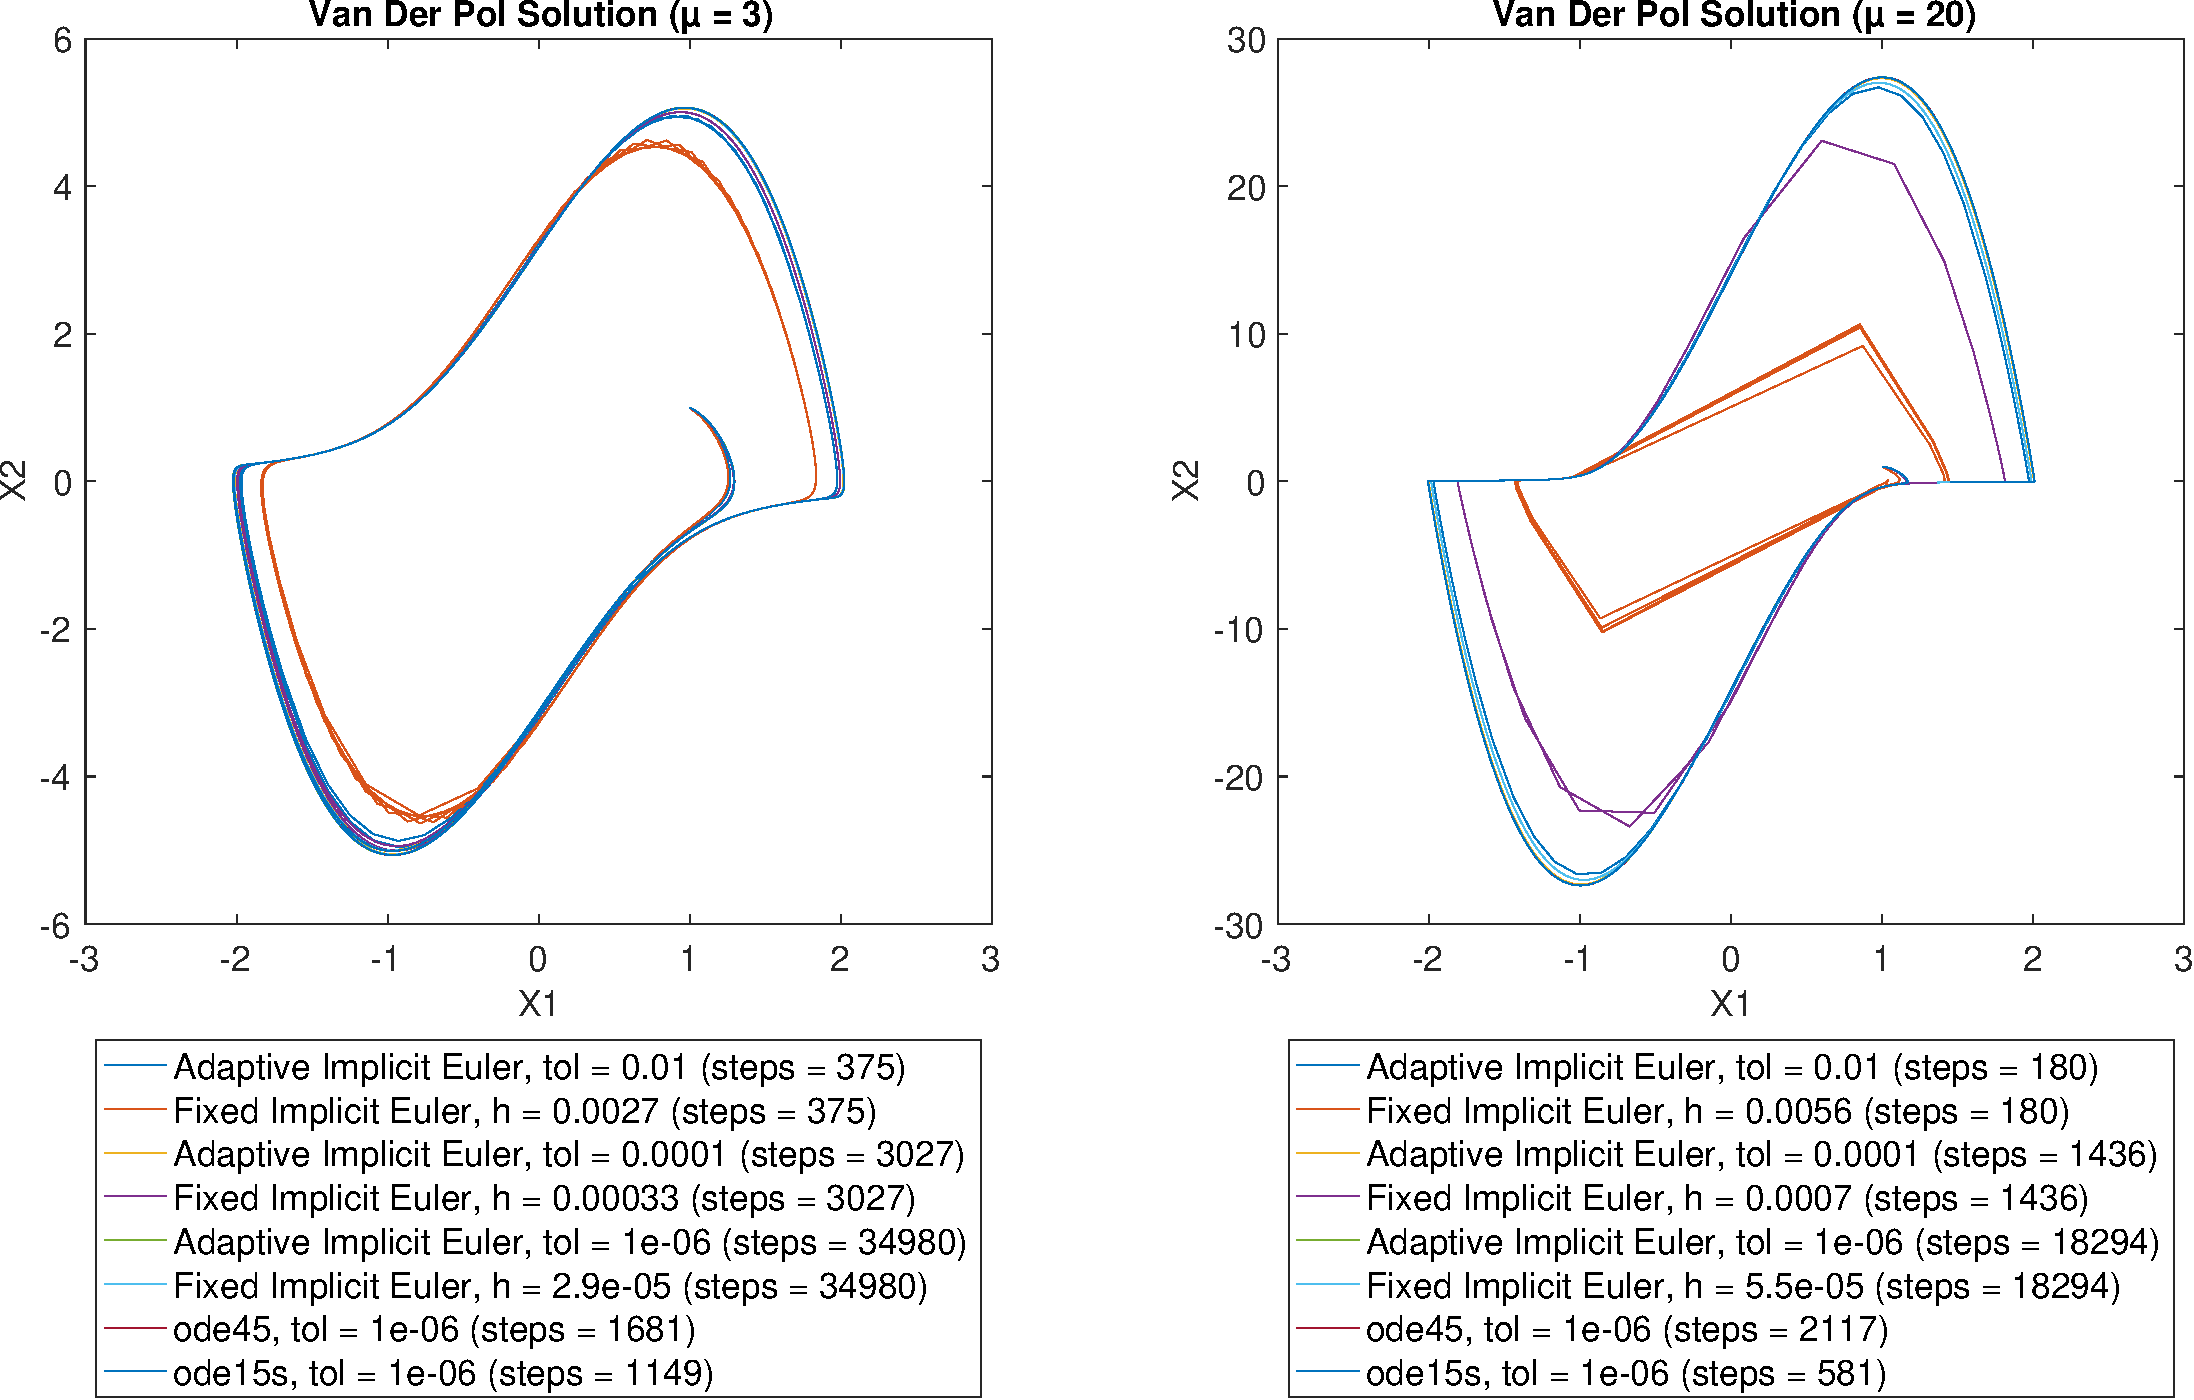
\includegraphics[width=\textwidth]{plots/3_4main.pdf}
    \caption{Implicit Euler method tested on the Van der Pol problem. Both an adaptive step size strategy with tolerance = 0.01 and a fixed step size strategy fixed to equal number of steps is applied.}
    \label{fig:2_4a}
\end{figure}


\subsection{Discussion of interface}
The methods have been implemented in a similar fashion to MATLAB's ode45 and ode15s for comparison purposes. For better comparison of fixed vs. adaptive step size, the implementation of the fixed step size was designed to be able to take a $N$ number of steps as input.
\clearpage
\section{Solvers for SDEs}
Considering now the stochastic differential equation (SDE)
$$
d x(t)=f\left(t, x(t), p_{f}\right) d t+g\left(t, x(t), p_{g}\right) d \omega(t) \quad d \omega(t) \sim N_{i i d}(0, I \Delta t)
$$

where $x \in \mathbb{R}^{n_{x}}$ and $\omega$ is a multivariate stochastic variable following a Wiener Process. The first term \textit{f()} is commonly referred to as the \textit{drift term} and the ladder term \textit{g()} is commonly referred to as the \textit{diffusion term}. The ODE is a particular case of an SDE where $g() = 0$. If the diffusion $g()$ does not change for different values of $x(t)$ the diffusion is said to be \textit{state independent} and said to be \textit{state dependent} otherwise.

\subsection{Wiener Process}
The Wiener Process is a stochastic process (a sequence of stochastic variables) realised from identical and independent Gaussian distributions with 0 mean and variance increasing with time \textit{dt}. It therefore models continuous perturbations allowing for greater variation when more time has passed. Using the reparametrization trick one can pull out the variance and use the standard Gaussian. It is implemented in MATLAB as follows:

\begin{adjustwidth*}{0cm}{-0.4cm}
\begin{lstlisting}[frame=single, language=Matlab,caption=Wiener Process, label=LittleWiener]
function [W,Tw,dW] = StdWienerProcess(T,N,nW,Ns,seed)
if nargin == 4
    rng(seed);
end
dt = T/N; % Fixed step size
dW = sqrt(dt)*randn(nW,N,Ns);
W = [zeros(nW,1,Ns) cumsum(dW,2)];
Tw = 0:dt:T;
\end{lstlisting}
\end{adjustwidth*}

\subsection{Explicit-Explicit (Euler-Maruyama)}
An SDE solver has to address both the drift term and the diffusion term. By linearity of integration the integral can be split into two integrals

\begin{equation}
\boldsymbol{x}\left(t_{k+1}\right)-\boldsymbol{x}\left(t_{k}\right)=\int_{t_{k}}^{t_{k+1}} f(\boldsymbol{x}(t)) d t+\int_{t_{k}}^{t_{k+1}} g(\boldsymbol{x}(t)) d \boldsymbol{\omega}(t)
\end{equation}

The drift term can be solved by a Riemann integral for which we have numerous approximation methods normally associated with ODEs. The diffusion term however requires an Itô integral \cite{JrgensenScientificEquationsd}. "Explicit-Explicit" refers to solving the drift term with an explicit method and the diffusion term with an explicit method. We will use the Euler-Maruyama for approximating the solution to the SDE:

\begin{equation}
\boldsymbol{x}_{k+1}-\boldsymbol{x}_{k}=f\left(\boldsymbol{x}_{k}\right) \Delta t_{k}+g\left(\boldsymbol{x}_{k}\right) \Delta \boldsymbol{w}_{k}
\end{equation}

Where we will use a fixed step size $\Delta t_k = \Delta t$. Note how the SDE is discretized as usual. It is based on a forward step $f\left(\boldsymbol{x}_{k}\right)$ for the drift and a forward step $g\left(\boldsymbol{x}_{k}\right)$ for the diffusion, i.e. Explicit-Explicit. The MATLAB implementation is found below.

\begin{adjustwidth*}{0cm}{-0.4cm}
\begin{lstlisting}[frame=single, language=Matlab,caption=Euler-Maruyama, label=hnrkmdsen]
function X = SDEsolverExplicitExplicit(ffun,gfun,T,x0,W,varargin)
N = length(T);
nx = length(x0);
X = zeros(nx,N);

X(:,1) = x0;
for k=1:N-1
    f = feval(ffun,T(k),X(:,k),varargin{:});
    g = feval(gfun,T(k),X(:,k),varargin{:});
    dt = T(k+1)-T(k); % Allow for varying step size
    dW = W(:,k+1)-W(:,k);
    psi = X(:,k) + g*dW; % The diffusion/pertubation 
    X(:,k+1) = psi + f*dt; % Add the drift
end
\end{lstlisting}
\end{adjustwidth*}

\subsection{Implicit-Explicit}
Now the drift term can also be solved by an Implicit Euler method as shown in Section 3. The approximation to the SDE is then

\begin{equation}
\boldsymbol{x}_{k+1}=\boldsymbol{x}_{k}+f\left(\boldsymbol{x}_{k+1}\right) \Delta t_{k}+g\left(\boldsymbol{x}_{k}\right) \Delta \boldsymbol{w}_{k}
\end{equation}

Where we will use a fixed step size $\Delta t_k = \Delta t$. Note how it is based on $f\left(\boldsymbol{x}_{k+1}\right)$ for the drift, where $x_{k+1}$ is unknown and calculated implicitly. The step for the diffusion is an explicit forward step $g\left(\boldsymbol{x}_{k}\right)$ for the diffusion. In other words, the method is an Implicit-Explicit method. The MATLAB implementation is found below.

\begin{adjustwidth*}{0cm}{-0.4cm}
\begin{lstlisting}[frame=single, language=Matlab,caption=Implicit-Explicit, label=implicitexplicit]
function X=SDEsolverImplicitExplicit(ffun,gfun,T,x0,W,tol,varargin)
maxit = 100;

N = length(T);
nx = length(x0);
X = zeros(nx,N);

X(:,1) = x0;
k=1;
[f,~] = feval(ffun,T(k),X(:,k),varargin{:});
for k=1:N-1
    g = feval(gfun,T(k),X(:,k),varargin{:});
    dt = T(k+1)-T(k);
    dW = W(:,k+1)-W(:,k);
    psi = X(:,k) + g*dW;
    xinit = psi + f*dt;
    [X(:,k+1),f,~] = SDENewtonSolver(...
            ffun,...
            T(:,k+1),dt,psi,xinit,...
            tol,maxit,varargin{:});
end
\end{lstlisting}
\end{adjustwidth*}

As with the Implicit Euler in Section 3, it is based on Newton's method for finding a root of the residual function by iteratively taking steps along the Jacobian evaluated in the current iteration. The implementation is seen in Listing \ref{newtonsde}.

\begin{adjustwidth*}{0cm}{-0.4cm}
\begin{lstlisting}[frame=single, language=Matlab,caption=Newton's Method for SDEs, label=newtonsde]
function [x,f,J] = SDENewtonSolver(ffun,t,dt,psi,xinit,tol,maxit,varargin)
I = eye(length(xinit));
x = xinit;
[f,J] = feval(ffun,t,x,varargin{:});
R = x - f*dt - psi;

it=1;
while( (norm(R,'inf') > tol) && (it <= maxit) )
    dRdx = I - J*dt;
    mdx = dRdx\R;
    x = x - mdx;
    [f,J] = feval(ffun,t,x,varargin{:});
    R = x - f*dt - psi;
    it = it+1;
end
\end{lstlisting}
\end{adjustwidth*}


\subsection{Description of implementations}
Implementations and methods has already been described and code included under the relevant methods in Section 4.2 and 4.3.

\subsection{Van der Pol}
In this section the above listed MATLAB implementations are tested on the Van der Pol problem. Until now we have only modelled a deterministic drift. The Van der Pol problem is now extended with a diffusion term. Two different diffusion functions will be tested, a state independent and state dependent respectively:

\begin{align*}
    & g(t, \boldsymbol{x}(t), \sigma) = [0, \sigma]^T \quad (1) \\
    & g(t, \boldsymbol{x}(t), \sigma) = [0, \sigma (1 + x_1(t)^2)]^T \quad (2)
\end{align*}

Resulting in SDE version (1) of the Van der Pol problem:

\begin{equation}
\label{sde1}
\begin{aligned}
d x_{1}(t) &=x_{2}(t) d t \\
d x_{2}(t) &=\left[\mu\left(1-x_{1}(t)^{2}\right) x_{2}(t)-x_{1}(t)\right] d t+\sigma d \omega(t)
\end{aligned}
\end{equation}

And SDE version (2) of the Van der Pol problem:

\begin{equation}
\label{sde1}
\begin{aligned}
&d x_{1}(t)=x_{2}(t) d t \\
&d x_{2}(t)=\left[\mu\left(1-x_{1}(t)^{2}\right) x_{2}(t)-x_{1}(t)\right] d t+\sigma\left(1+x_{1}(t)^{2}\right) d \omega(t)
\end{aligned}
\end{equation}

And fixed step size of $\Delta t = h = 0.001$ is used.







\\\

\textbf{Version (1) - state independent diffusion}
In this section, equation (\ref{sde1}) is solved for realizations with $\sigma \in \{A,B,C,D\}$:

\begin{figure}
    \centering
    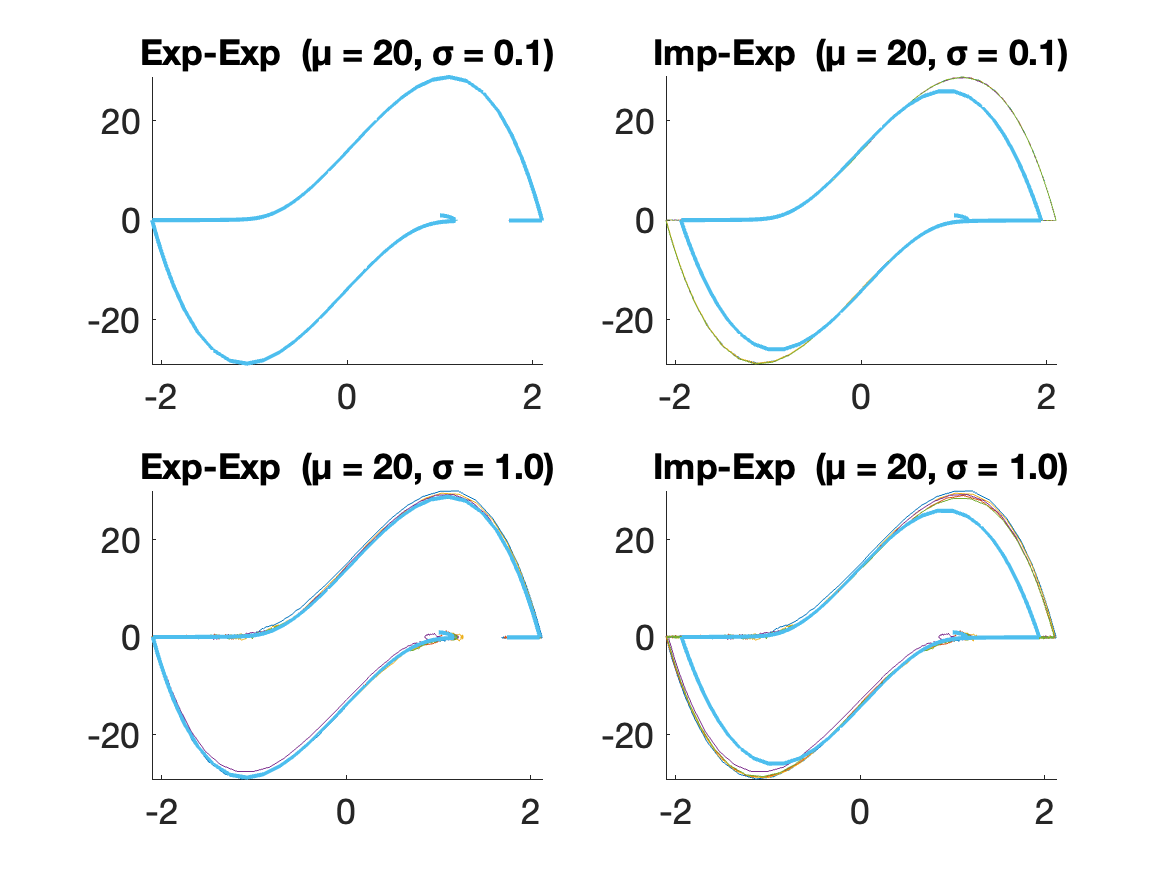
\includegraphics[width=\textwidth]{plots/4a.pdf}
    \caption{cap}
    \label{fig:4a}
\end{figure}

\begin{figure}
    \centering
    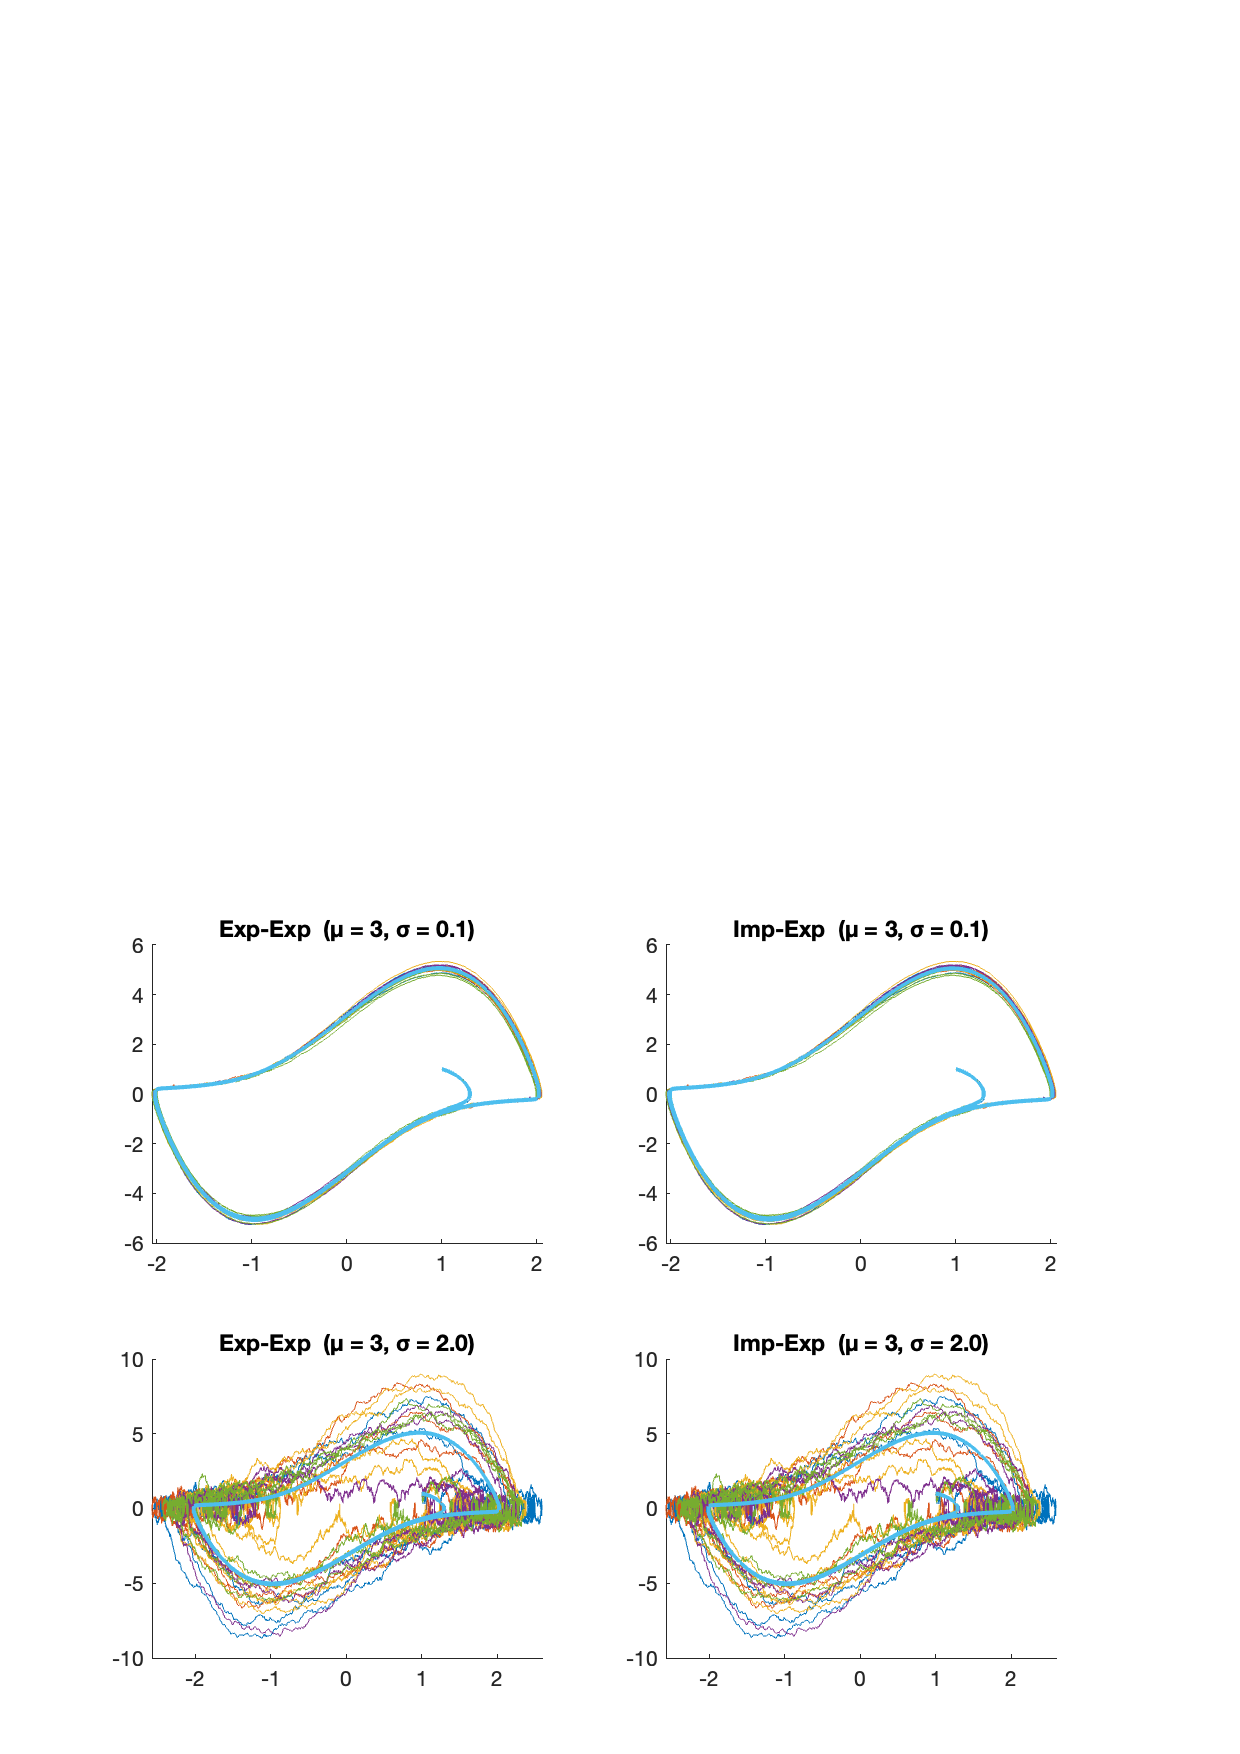
\includegraphics[width=\textwidth]{plots/4b.pdf}
    \caption{cap}
    \label{fig:4b}
\end{figure}
\clearpage
\section{Classical Runge-Kutta method}

\subsection{Description of Runge-Kutta}
As all other numerical solvers we have seen, Runge-Kutta discretizes the continous ODE by iteratively computing $x_{n+1}$ from $x_n$, i.e. using a finite-difference approximation. But whereas the previous methods take one long step from $x_n$ to $x_{n+1}$, Runge-Kutta is based on first taking multiple in-between steps $X_j$ for $j=1..s$ where $s$ is the number of stages. The computation $x_{n+1}$ is then computed as an weighted average of the stages. The higher number of stages, the higher is the order of the method and therefore also higher the accuracy. For error estimation instead of using step doubling, a higher order method is typically used ($\hat{x}_{n+1}$). The error is the estimated as $e_{n+1}=x_{n+1}-\hat{x}_{n+1}$. All in all the equations are denoted \cite{JrgensenRunge-KuttaEquations}:\\
\underline{Stages}

\begin{equation}
\label{eq:RKgeneral1}
\begin{aligned}
&T_{i}=t_{n}+c_{i} \Delta t_n \quad i=1,2, \ldots, s\\
&X_{i}=x_{n}+\Delta t_n \sum_{j=1}^{s} a_{i j} f\left(T_{j}, X_{j}\right) \quad i=1,2, \ldots, s
\end{aligned}
\end{equation}

Where the full \underline{next step} from $x_n$ to $x_{n+1}$ is calculated by

\begin{equation}
\label{eq:RKgeneral2}
\begin{aligned}
&t_{n+1}=t_{n}+\Delta t_n \\
&x_{n+1}=x_{n}+\Delta t_n \sum_{j=1}^{s} b_{j} f\left(T_{j}, X_{j}\right) \\
&\hat{x}_{n+1}=x_{n}+\Delta t_n \sum_{j=1}^{s} \hat{b}_{j} f\left(T_{j}, X_{j}\right) \\
&e_{n+1}=x_{n+1}-\hat{x}_{n+1}=\Delta t_n \sum_{j=1}^{s} d_{j} f\left(T_{j}, X_{j}\right) \quad d_{j}=b_{j}-\hat{b}_{j}
\end{aligned}
\end{equation}

The Explict and Implicit Euler methods are particular cases of the Runge-Kutta with s=1.

\\\

\textbf{Classical Runge-Kutta}\\
One intuitive idea is to let the stages only depend on previous $X_j$'s leading to Explicit Runge-Kutta methods. The Classical Runge-Kutta is such a method. Additionally, it is a 4 stage method where the different coefficients is chosen as summarized by this Butcher Tableau \cite{JrgensenRunge-KuttaEquations}

$$
\begin{array}{c|cccc}
0 & & & & \\
\frac{1}{2} & \frac{1}{2} & & & \\
\frac{1}{2} & 0 & \frac{1}{2} & & \\
1 & 0 & 0 & 1 & \\
\hline \mathrm{X} & \frac{1}{6} & \frac{1}{3} & \frac{1}{3} & \frac{1}{6}
\end{array}
$$

Which means that $x_{n+1}$ is iteratively calculated by

\begin{equation*}
\begin{array}{ll}
T_{1}=t_{n} & X_{1}=x_{n} \\
T_{2}=t_{n}+\frac{1}{2} \Delta t_n & X_{2}=x_{n}+\Delta t_n \frac{1}{2} f\left(T_{1}, X_{1}\right) \\
T_{3}=t_{n}+\frac{1}{2} \Delta t_n & X_{3}=x_{n}+\Delta t_n \frac{1}{2} f\left(T_{2}, X_{2}\right) \\
T_{4}=t_{n}+\Delta t_n & X_{4}=x_{n}+\Delta t_n f\left(T_{3}, X_{3}\right)
\end{array}
\end{equation*}

\begin{equation}
\label{eq:cRK1}
\begin{aligned}
&t_{n+1}=t_{n}+\Delta t_n \\
&x_{n+1}=x_{n}+\Delta t_n\left(\frac{1}{6} f\left(T_{1}, X_{1}\right)+\frac{1}{3} f\left(T_{2}, X_{2}\right)+\frac{1}{3} f\left(T_{3}, X_{3}\right)+\frac{1}{6} f\left(T_{4}, X_{4}\right)\right)
\end{aligned}
\end{equation}

The classical Runge-Kutta has no embedded method for error estimation.

\subsection{MATLAB implementation fixed step size}
The above mentioned classical Runge-Kutta method is implemented in MATLAB with a fixed step size $\Delta t_n = h$. For readability, the classical Runge-Kutta step is implemented separately in listing \ref{ERKpars} to be used in listing \ref{ERK} and \ref{ERKadapt}. The classical Runge-Kutta step is simply the implementation of equation \ref{eq:cRK1}.

\begin{adjustwidth*}{0cm}{-0.4cm}
\begin{lstlisting}[frame=single, language=Matlab,caption=Classical Runga-Kutta Step, label=ERKpars]
function [t1, x1] = ClassicalRungeKuttaStep(...
    fun,t,x,f,h,varargin)
h2 = 0.5*h;
alpha = h/6;
beta = h/3;

T1 = t;
X1 = x;
F1 = f;

T2 = x+h2;
X2 = x+h2*F1;
F2 = feval(fun,T2,X2,varargin{:});

T3 = T2;
X3 = x+h2*F2;
F3 = feval(fun,T3,X3,varargin{:});

T4 = t+h;
X4 = x+h*F3;
F4 = feval(fun,T4,X4,varargin{:});

t1 = T4;
x1 = x + alpha*(F1+F4) + beta*(F2+F3);
\end{lstlisting}
\end{adjustwidth*}

The classical Runge-Kutta with fixed step size is simply taking steps (listing \ref{ERKpars}) in the specified range as seen in listing \ref{ERK}.

\begin{adjustwidth*}{0cm}{-0.4cm}
\begin{lstlisting}[frame=single, language=Matlab,caption=Classical Runge-Kutta with fixed step size, label=ERK]
function [T,X] = ClassicalRungeKuttaFixedStep(...
    fun,tspan,x0,h,varargin)
% Integration interval
t0 = tspan(1);
tf = tspan(2);

% Initial conditions
t = t0;
x = x0;

T = t;
X = x';

%% Algo
while t < tf
    if (t+h > tf)
        h = tf-t;
    end
    % f at x_n
    f = feval(fun, t,x,varargin{:});

    % Take step of size h to obtain x_{n+1}
    [t, x] = ClassicalRungeKuttaStep(...
        fun,t,x,f,h,varargin{:});

     T = [T; t];
     X = [X; x'];
end
\end{lstlisting}
\end{adjustwidth*}



\subsection{MATLAB implementation adaptive step size}
Similarly to listing \ref{ERK}, the below implementation of an adaptive step size uses classical Runge-Kutta steps (listing \ref{ERKpars}) and adaptively changes the step size relative to specified tolerances. The error estimation is based on step doubling, iteratively decreasing the step size until the error (as estimated by taking the two half steps) is below specified tolerances. The step doubling procedure is described in full detail in Section \ref{sec:stepdoubling}. The implementation of the adaptive classical Runge-Kutta is seen in listing \ref{ERKadapt}.

\begin{adjustwidth*}{0cm}{-0.4cm}
\begin{lstlisting}[frame=single, language=Matlab,caption=Explicit Runge-Kutta with adaptive step size, label=ERKadapt]
function [T,X,H] = ClassicalRungeKuttaAdaptiveStep(...
    fun,tspan,x0,h0,abstol,reltol,varargin)
epstol = 0.8;
kpow = 0.2; % 1/(order+1)
facmin = 0.1;
facmax = 5;

% Integration interval
t0 = tspan(1);
tf = tspan(2);

% Initial conditions
t = t0;
h = h0;
x = x0;

H = h;
T = t;
X = x';

%% Algo
while t < tf
    if (t+h > tf)
        h = tf-t;
    end
    f = feval(fun, t,x,varargin{:});

    AcceptStep = false;
    while ~AcceptStep
        % Take step of size h
        [t1, x1] = ClassicalRungeKuttaStep(...
            fun,t,x,f,h,varargin{:});

        % Take step of size h/2
        hm=0.5*h;
        [tm, xm] = ClassicalRungeKuttaStep(...
            fun,t,x,f,h,varargin{:});
        
        fm = feval(fun,tm,xm,varargin{:});
        [t1hat, x1hat] = ClassicalRungeKuttaStep(...
            fun,tm,xm,fm,hm,varargin{:});

        % Error estimation
        e = x1hat-x1;
        r = max(abs(e) ./ max(abstol, abs(x1hat) .*reltol));

        AcceptStep = (r<=1.0);
        if AcceptStep
            t = t+h;
            x = x1hat;
              
            T = [T;t];
            X = [X;x'];
            H = [H;h]; % Save taken step sizes
        end
        % Asymptotic step size controller
        h = max(facmin,min((epstol/r)^kpow,facmax))*h;
    end
end
\end{lstlisting}
\end{adjustwidth*}

\subsection{Van der Pol}
Let us use the two numerical solvers for solving the Van der Pol problem defined as

\begin{equation}
\label{eq:vanderpol}
\begin{aligned}
&\dot{x}_{1}(t)=x_{2}(t) \\
&\dot{x}_{2}(t)=\mu\left(1-x_{1}(t)^{2}\right) x_{2}(t)-x_{1}(t)
\end{aligned}
\end{equation}


\subsubsection*{Fixed step size}
See Figure \ref{fig:5_4fix} for the solution using the fixed step size. Clearly there is an increasing precision for lowering the step size $h$. This is particularly the case for the stiff-problem ($\mu = 20$) where the solution quickly goes to $\infty$ for $h=0.1$.

\begin{figure}[htb]
    \centering
    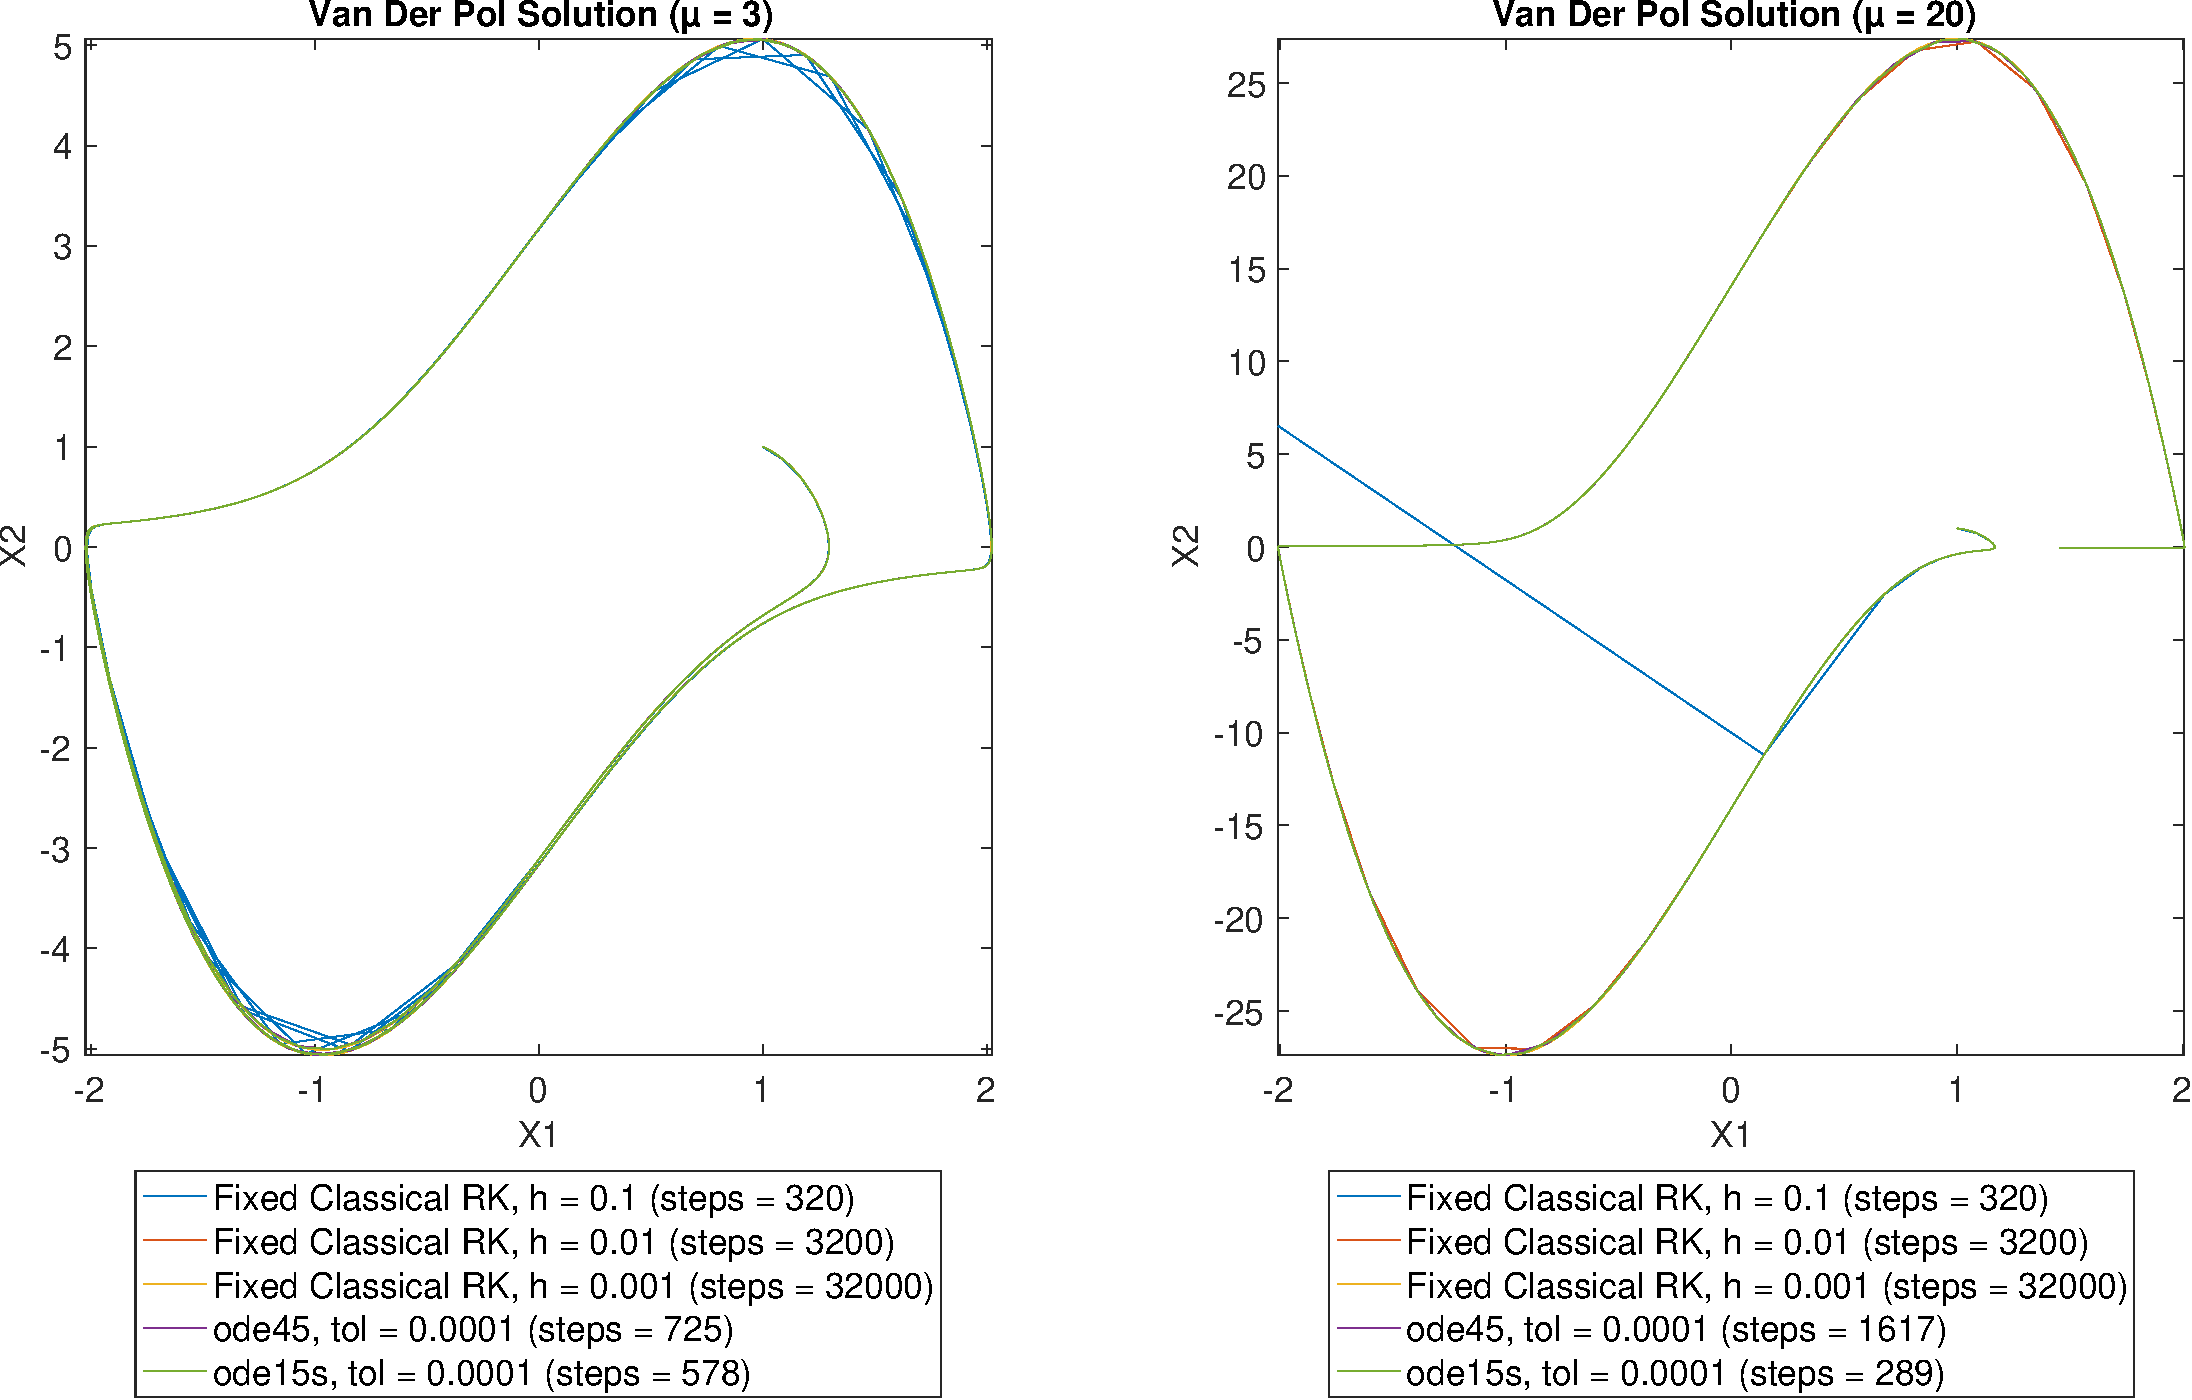
\includegraphics[width=\textwidth]{plots/5_4fix_a.pdf}
    \caption{Solution of Van der Pol using classical Runge-Kutta with fixed step size.}
    \label{fig:5_4fix}
\end{figure}







\subsubsection*{Adaptive step size}
The phase portrait of the solution from the solving the Van der Pol with the adaptive step size is seen in Figure \ref{fig:5_4}.

The corresponding $x_1$ and $x_2$ values over time is seen in Figure \ref{fig:5_4a}. Here, the stiffness of the problem with $\mu = 20$ is really clear. Interestingly, but not surprisingly, the step sizes drops accordingly to the stiff peaks of $x_2$ as seen in Figure \ref{fig:5_4b}.

\begin{figure}[h]
    \centering
    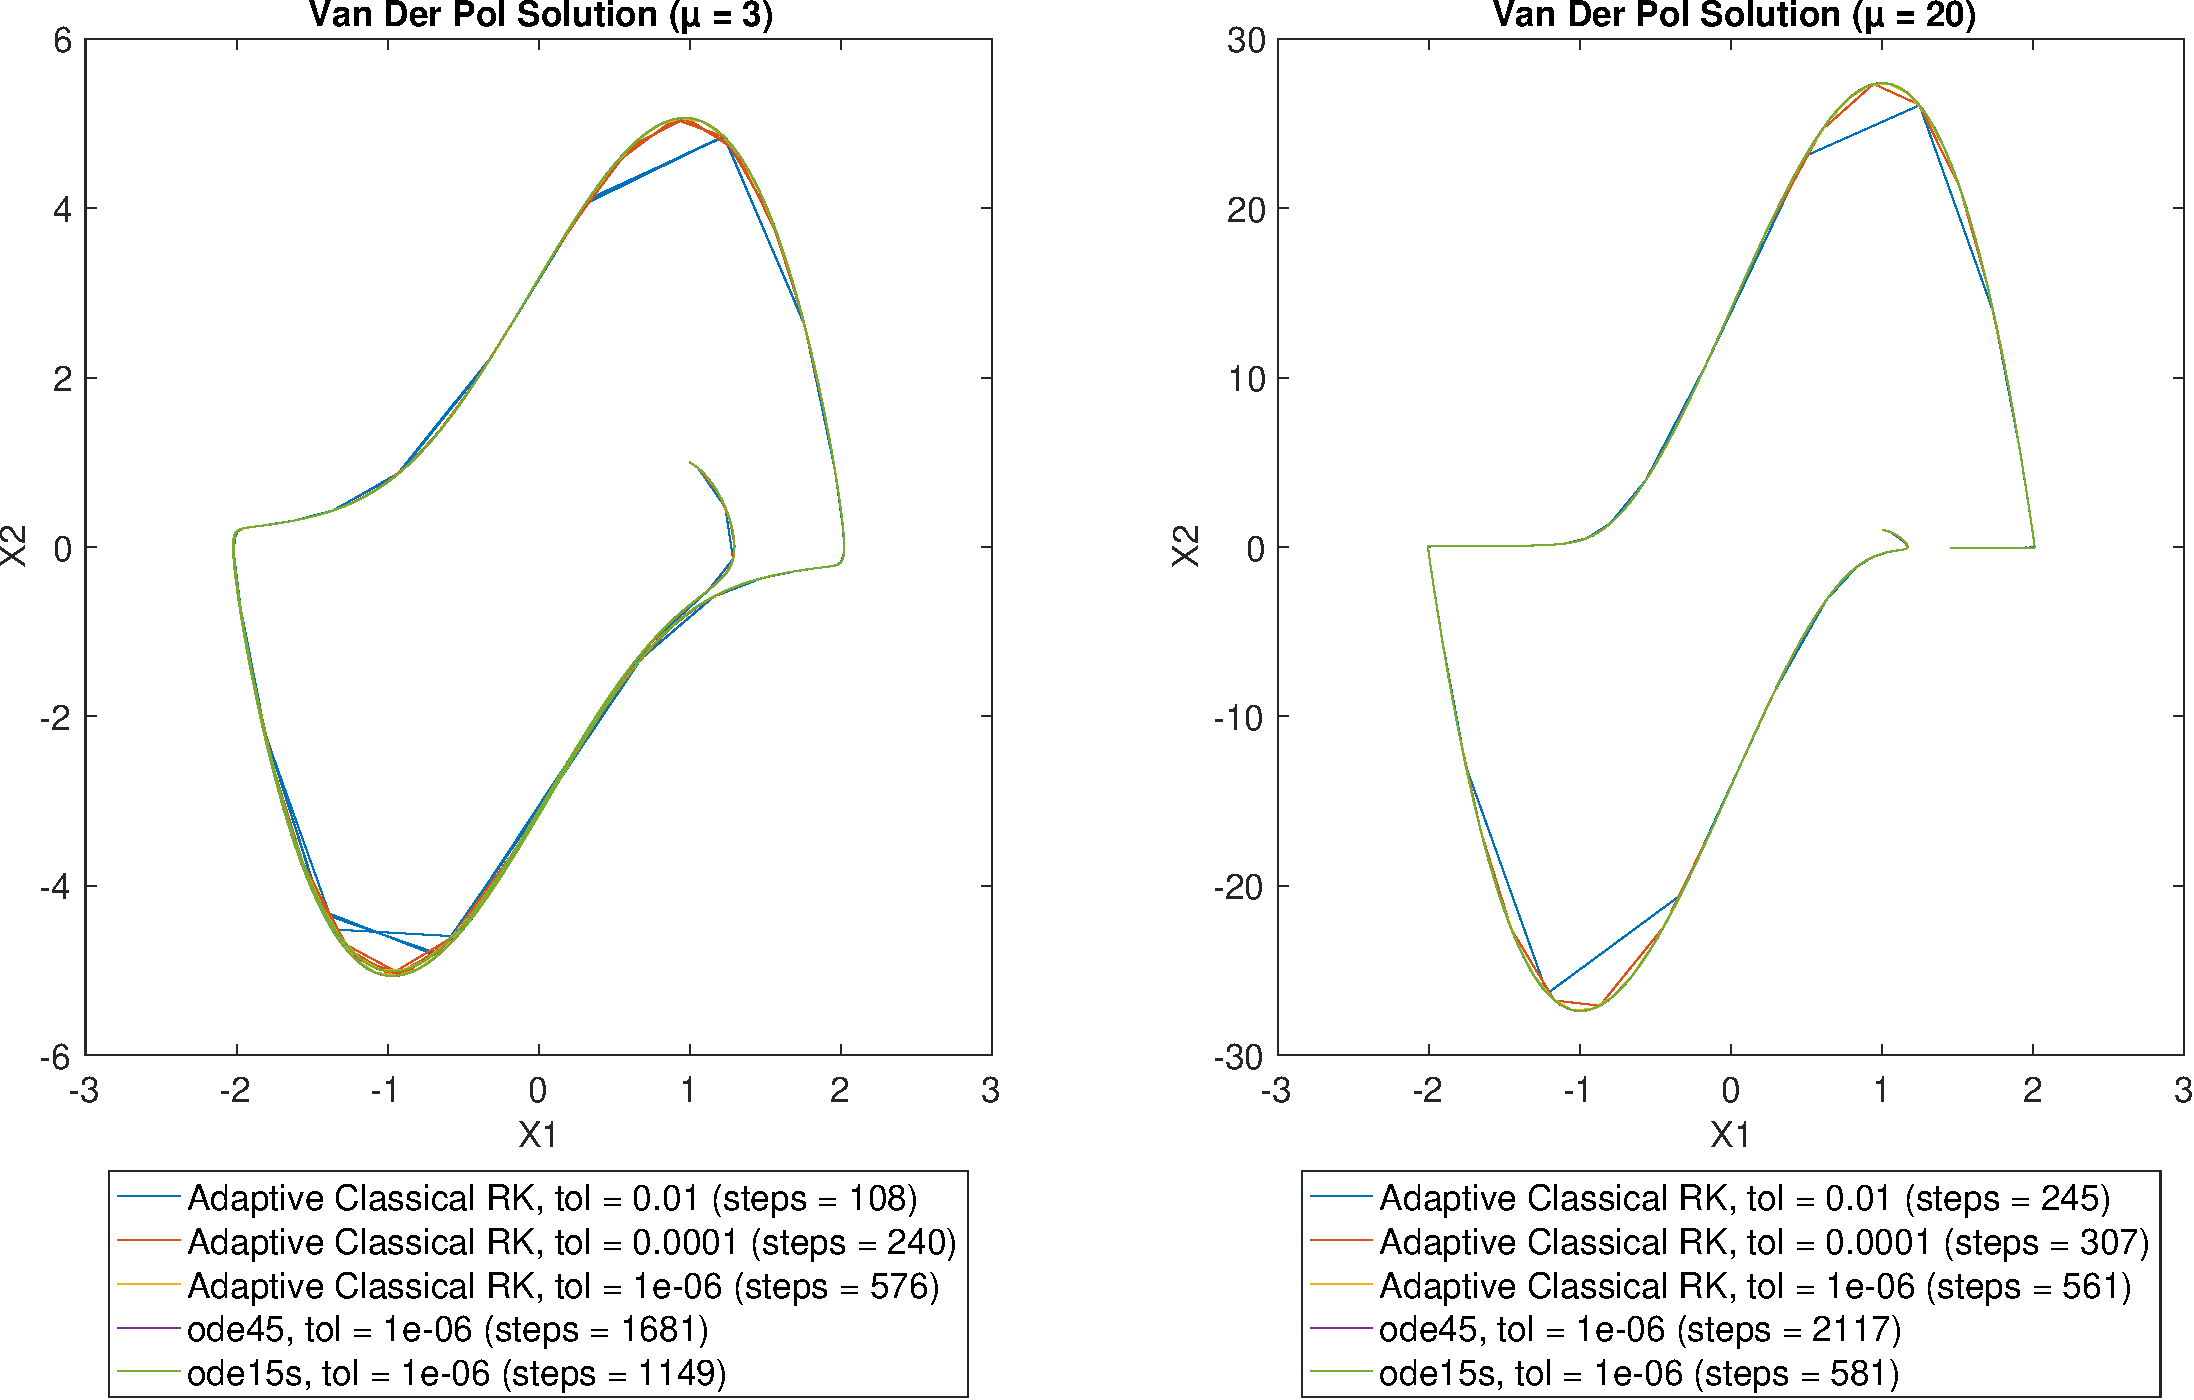
\includegraphics[width=\textwidth]{plots/5_4.pdf}
    \caption{Phase portrait of the solution of Van der Pol using classical Runge-Kutta with adaptive step size.}
    \label{fig:5_4}
\end{figure}






\begin{figure}[h]
\centering
\begin{subfigure}[b]{\textwidth}
   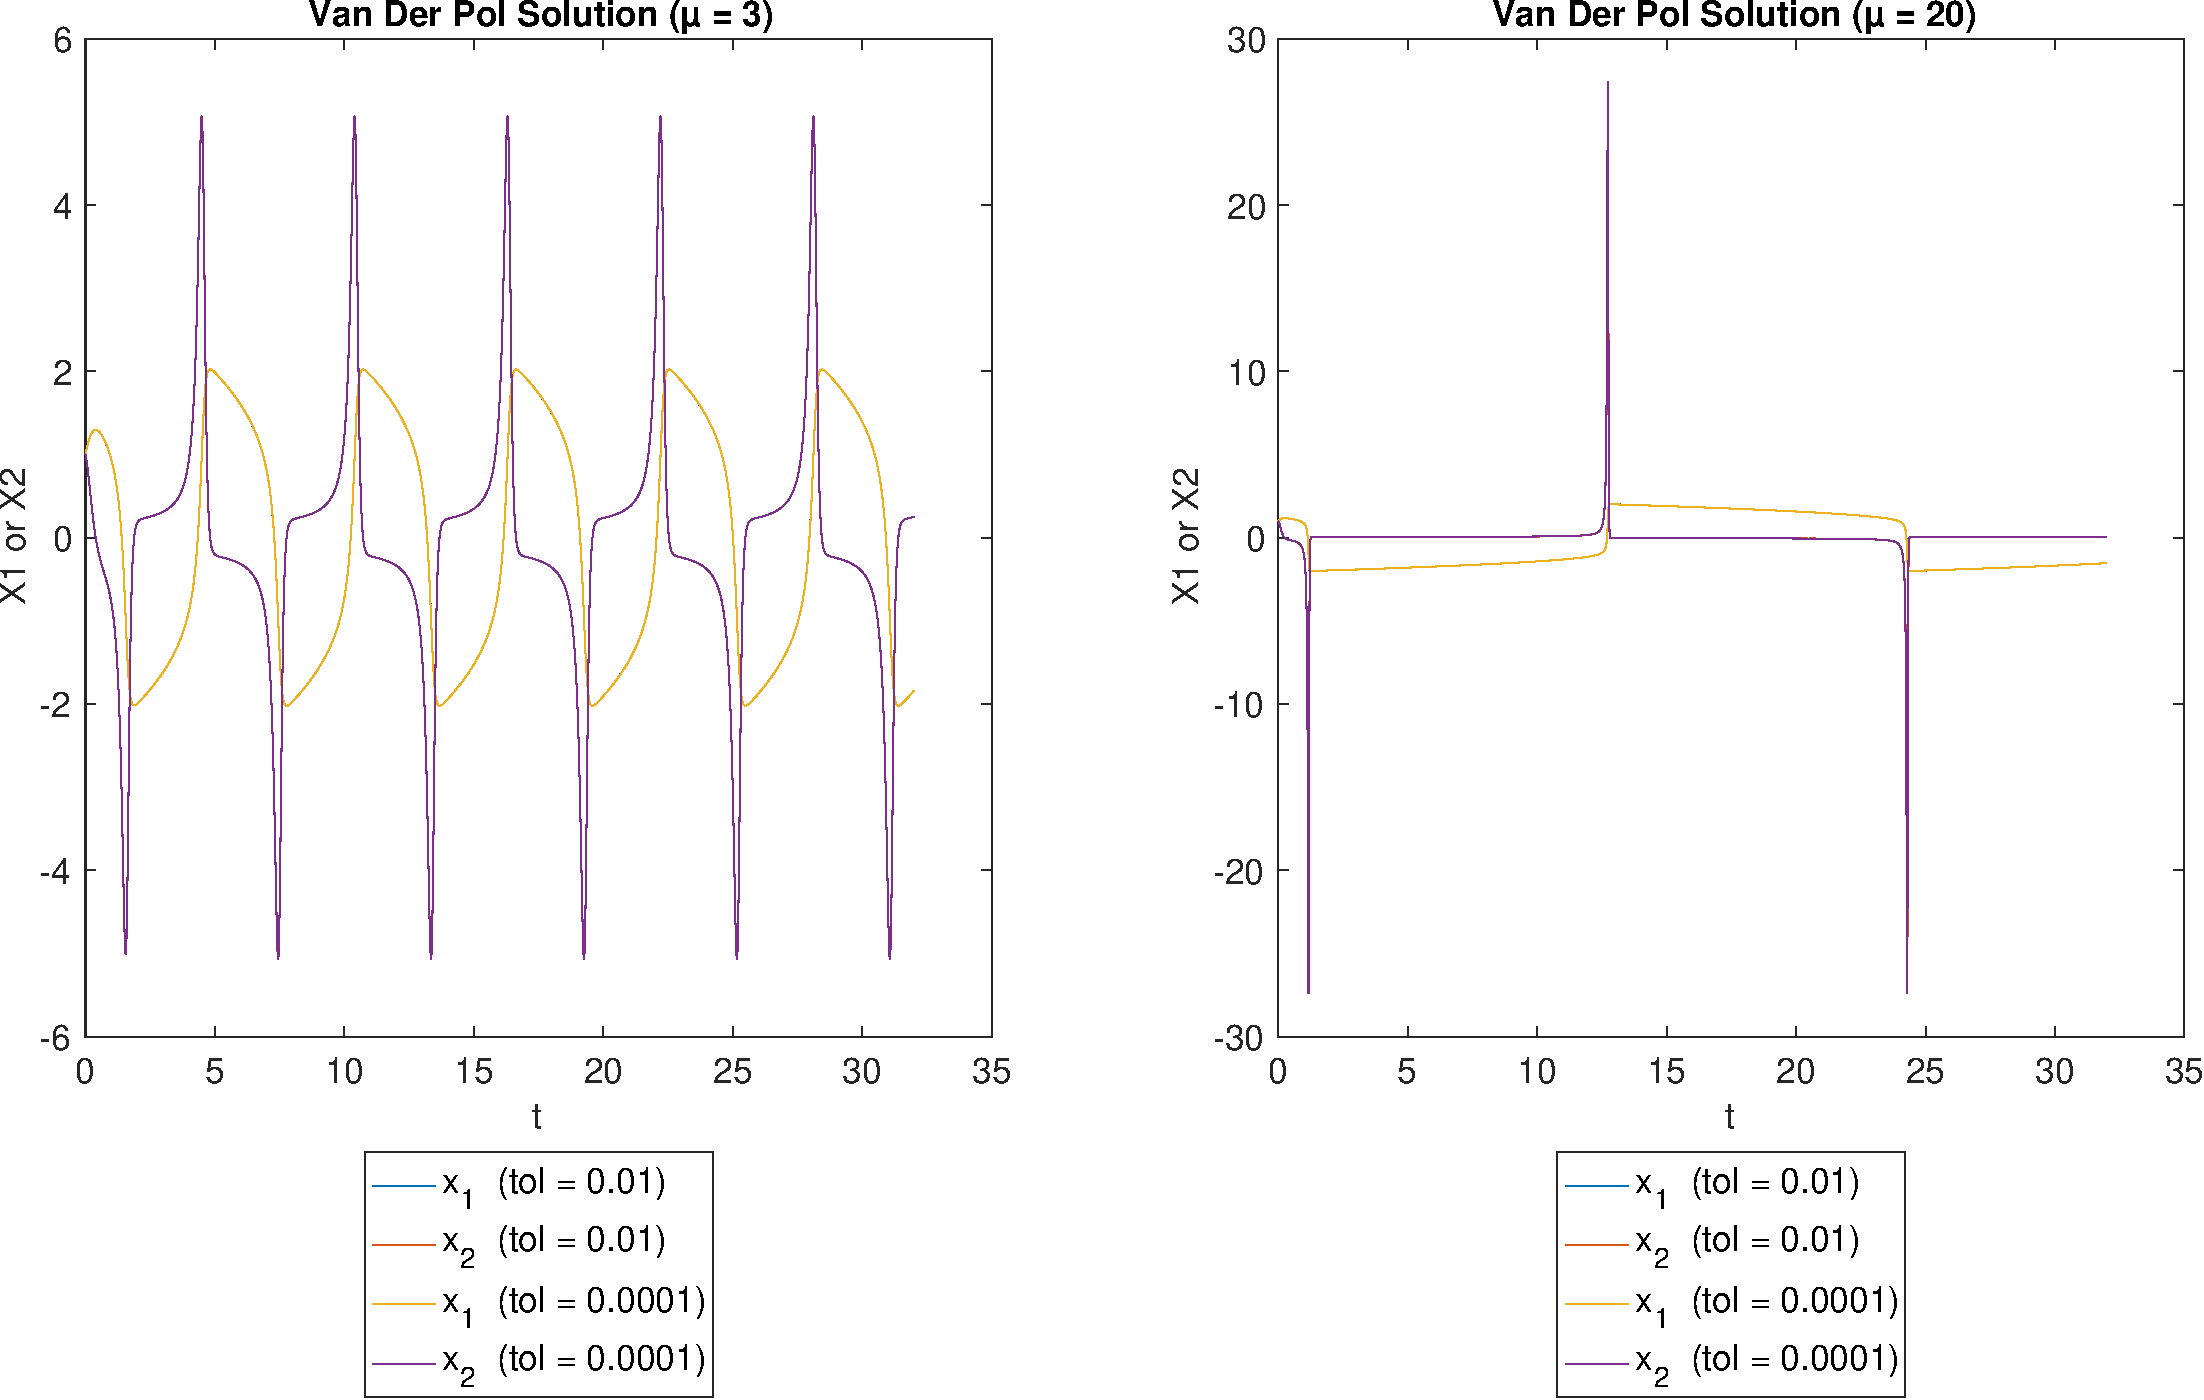
\includegraphics[width=1\linewidth]{plots/5_4a.pdf}
   \caption{}
   \label{fig:5_4a} 
\end{subfigure}

\begin{subfigure}[b]{\textwidth}
   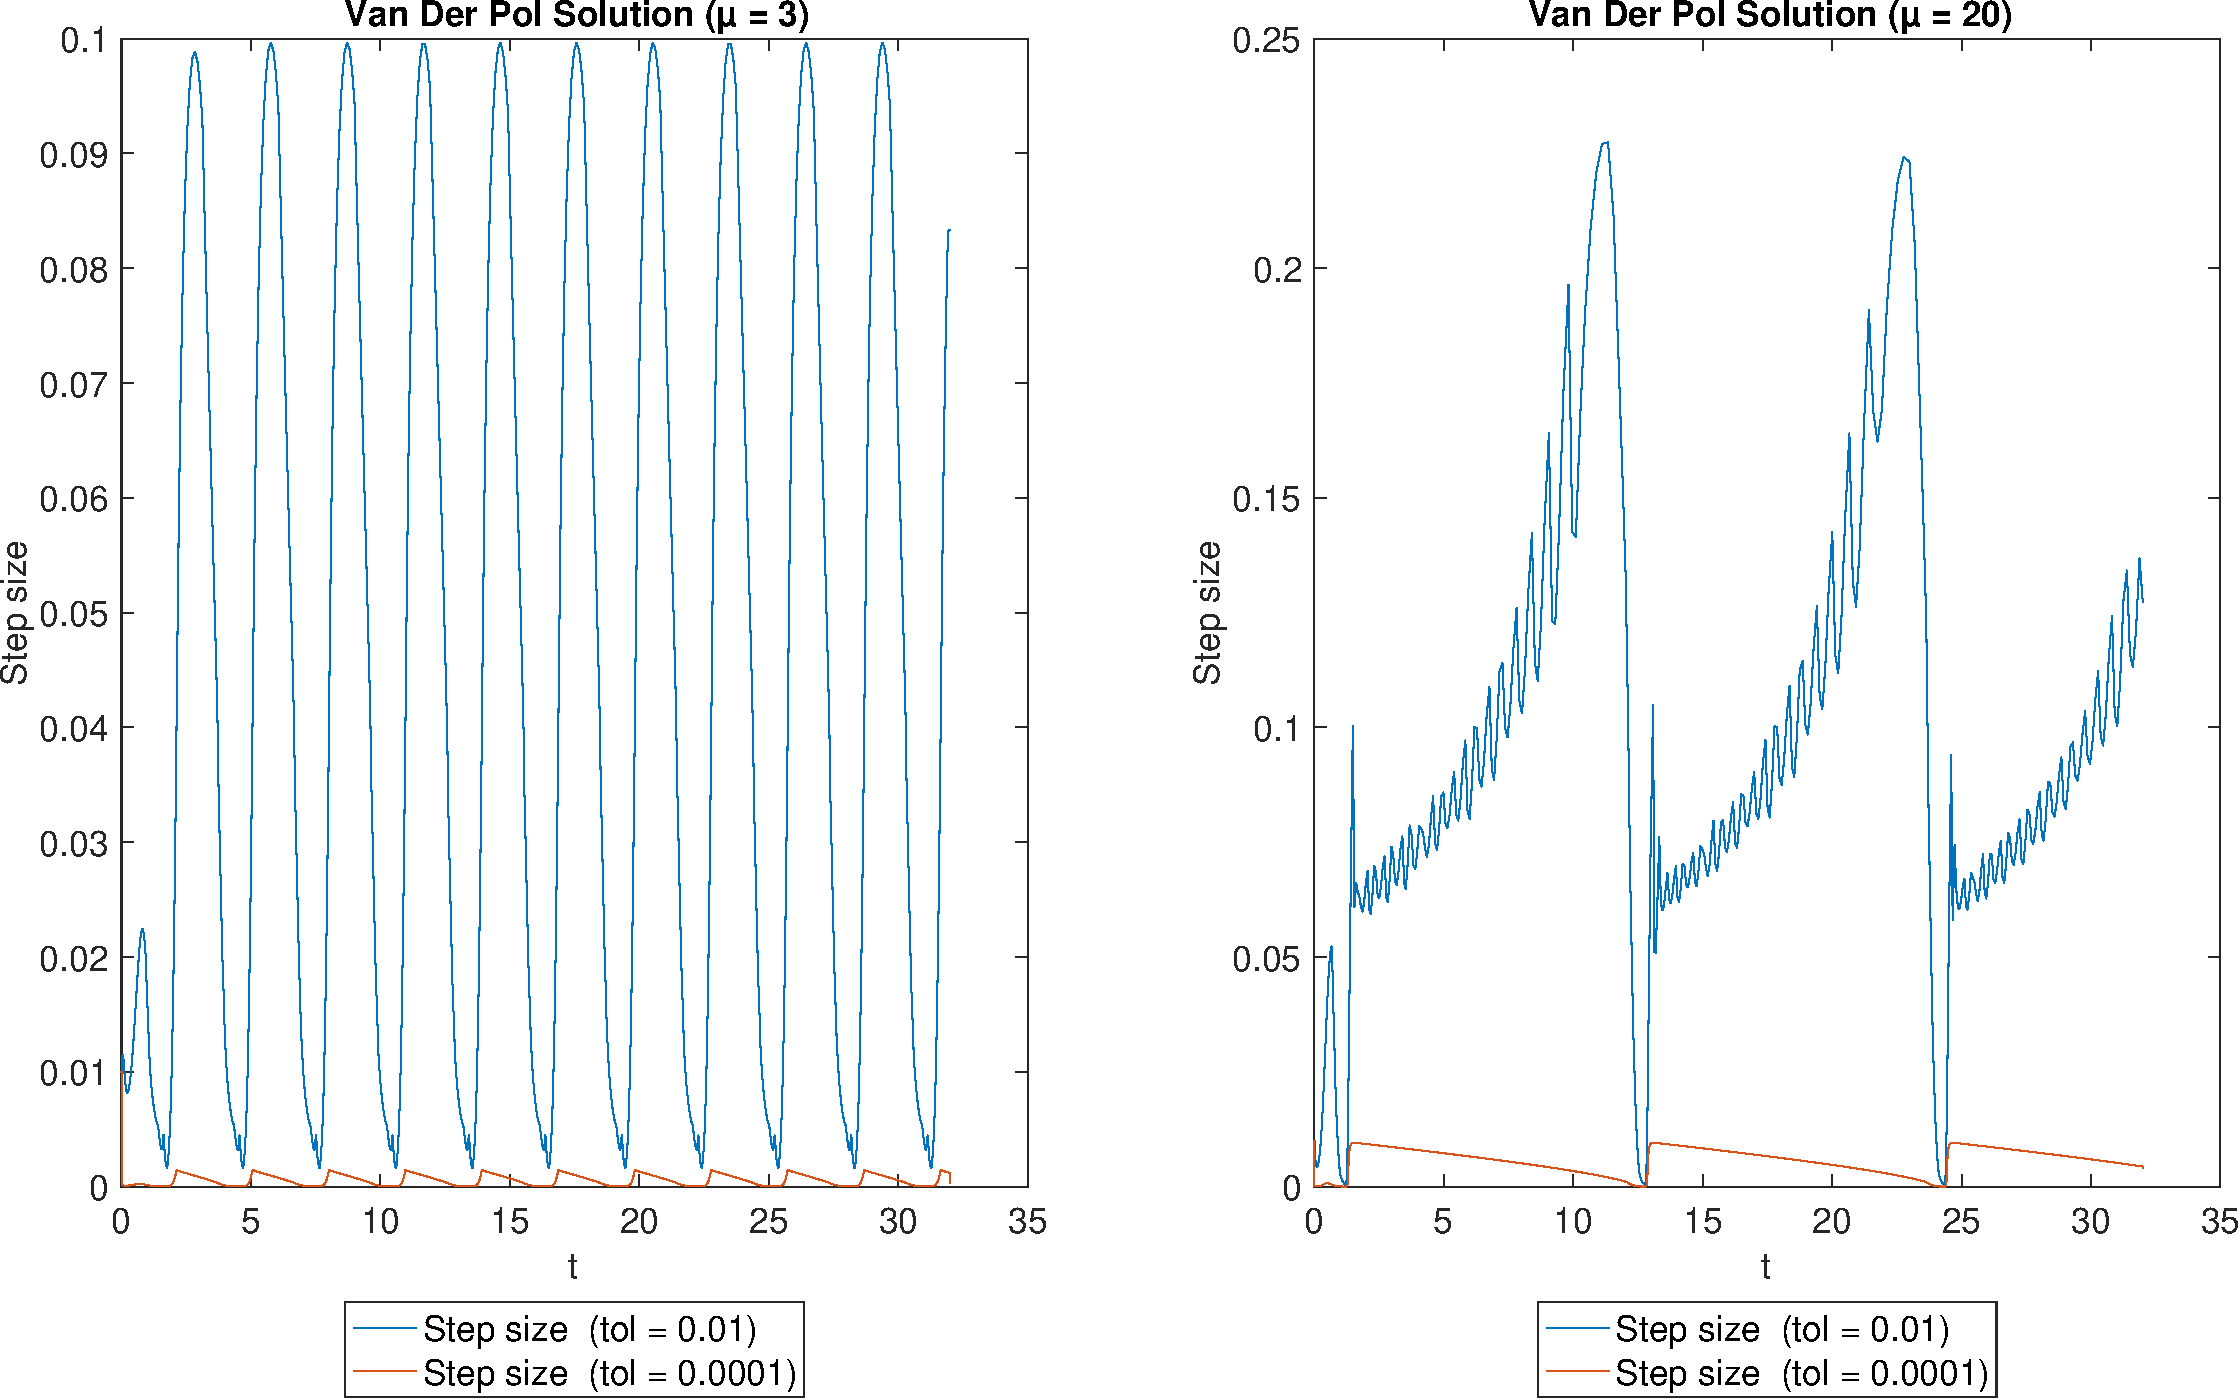
\includegraphics[width=1\linewidth]{plots/5_4b.pdf}
   \caption{}
   \label{fig:5_4b}
\end{subfigure}

\caption[Two numerical solutions]{(a) Solved $x_1$ and $x_2$ of the Van der Pol using classical Runge-Kutta with adaptive step size. (b) Corresponding step sizes.}
\end{figure}



\subsection{Discussion of interface}
In this sections we have seen the classical Runge-Kutta method, where the calculation of $x_{k+1}$ is done using 4 intermediate steps. Since the classical Runge-Kutta method is a very specific case of the general Runge-Kuta methods, it seems obvious to implement the more general family. That is what I did originally. But to show the classical Runge-Kutta more explicitly it was implemented directly\\
It was implemented in a similar fashion to MATLAB’s ode45 and ode15s for easy switching between solvers.

\clearpage


\blankpage
\section{ESDIRK23}

\begin{table}[H]
    \centering
\begin{tabular}{c|ccc}
0 & 0 & & \\
$c_{2}$ & $a_{21}$ & $\gamma$ & \\
1 & $b_{1}$ & $b_{2}$ & $\gamma$ \\
\hline$x_{n+1}$ & $b_{1}$ & $b_{2}$ & $\gamma$ \\
$\hat{x}_{n+1}$ & $\hat{b}_{1}$ & $\hat{b}_{2}$ & $\hat{b}_{3}$ \\
\hline$e_{n+1}$ & $d_{1}$ & $d_{2}$ & $d_{3}$
\end{tabular}
    \caption{Caption}
    \label{tab:my_label}
\end{table}


\begin{table}[H]
    \centering
\begin{tabular}{c|ccc}
0 & 0 & & \\
$2 - \sqrt{2}$ & $1 - \frac{\sqrt{2}}{2}$ & $1 - \frac{\sqrt{2}}{2}$ & \\
1 & $\frac{\sqrt{2}}{4}$ & $\frac{\sqrt{2}}{4}$ & $1 - \frac{\sqrt{2}}{2}$ \\
\hline$x_{n+1}$ & $\frac{\sqrt{2}}{4}$ & $\frac{\sqrt{2}}{4}$ & $1 - \frac{\sqrt{2}}{2}$ \\
$\hat{x}_{n+1}$ & $-\frac{\sqrt{2}}{12} + \frac{1}{3}$ & $\frac{\sqrt(2}{4}+\frac{1}{3}$ & $-\frac{\sqrt{2}}{6} + \frac{1}{3}$ \\
\hline$e_{n+1}$ & $\frac{\sqrt{2}}{3} - \frac{1}{3}$ & $-\frac{1}{3}$ & $\frac{2}{3} - \frac{\sqrt{2}}{3}$
\end{tabular}
    \caption{Caption}
    \label{tab:my_label}
\end{table}




Butcher
\begin{table}[H]
\centering
\begin{tabular}{c|ccc}
0 & 0 & 0 & 0 \\
$2-\sqrt{2}$ & $\frac{2-\sqrt{2}}{2}$  & $\frac{2-\sqrt{2}}{2}$ & 0 \\
$1$ & $\frac{\sqrt{2}}{4}$ & $\frac{\sqrt{2}}{4}$ & $\frac{2-\sqrt{2}}{2}$ \\ \hline
$x$ & $\frac{\sqrt{2}}{4}$ & $\frac{\sqrt{2}}{4}$ & $\frac{2-\sqrt{2}}{2}$ \\
$\hat{x}$ & $\frac{-\sqrt{2}+4}{12}$ & $\frac{3\sqrt{2}+4}{12}$ & $\frac{-\sqrt{2}+2}{6} $ \\ \hline
$e$ & $\frac{\sqrt{2}-1}{3}$ & $-\frac{1}{3}$ & $\frac{2-\sqrt{2}}{3}$
\end{tabular}
\caption{Buutcher}
\end{table}

input results from Maple.
\clearpage








% Bibliography
\section{Bibliography}
%\backmatter
\printbibliography

\end{document}